% ettdoc.tex V2.10, 19 June 2012

\documentclass[times]{ettauth}
\usepackage[toc,page]{appendix}
\usepackage{moreverb}

\usepackage[colorlinks,bookmarksopen,bookmarksnumbered,citecolor=red,urlcolor=red]{hyperref}

\usepackage{cite}
\newcommand\BibTeX{{\rmfamily B\kern-.05em \textsc{i\kern-.025em b}\kern-.08em
T\kern-.1667em\lower.7ex\hbox{E}\kern-.125emX}}

\def\volumeyear{2017}

\newcommand{\eg}{e.g., }
\newcommand{\ie}{i.e., }
\usepackage[linesnumbered,ruled,vlined]{algorithm2e}
\DeclareMathOperator*{\argmin}{\textbf{\upshape arg\,min}}
\DeclareMathOperator*{\argmax}{\textbf{\upshape arg\,max}}

\usepackage{times}
%\usepackage{mathptmx}
\usepackage{mathtools, cuted}
\usepackage[draft,nomargin,marginclue,footnote,silent]{fixme}
\setcounter{tocdepth}{2} %table of contents


\theoremstyle{mytheoremstyle}
\newtheorem{theorem}{Theorem}[section]

\theoremstyle{mytheoremstyle}
\newtheorem{corollary}{Corollary}[section]

\theoremstyle{mytheoremstyle}
\newtheorem{lemma}{Lemma}[section]

\newtheorem{mydef}{Definition}

\DeclareMathOperator*{\Max}{Max}
\DeclareMathOperator*{\Min}{Min}

\newcommand{\bigO}{\ensuremath{\mathcal{O}}}% big-O notation/symbol
\usepackage{subfigure}
\usepackage{adjustbox}
\usepackage{multirow}
\usepackage{enumitem}
\setlist[itemize]{leftmargin=*}
\setlist[enumerate]{wide=\parindent}
\usepackage[referable]{threeparttablex}
\renewlist{tablenotes}{enumerate}{1}
\makeatletter
\setlist[tablenotes]{label=\tnote{\alph*},ref=\alph*,itemsep=\z@,topsep=\z@skip,partopsep=\z@skip,parsep=\z@,itemindent=\z@,labelindent=\tabcolsep,labelsep=.2em,leftmargin=*,align=left,before={\footnotesize}}
\makeatother

\usepackage{graphicx}
\usepackage{sidecap}
\usepackage{kantlipsum} %<- For dummy text
\usepackage{mwe} %<- For dummy images
\usepackage{multirow}
\usepackage{multicol}
\usepackage{cleveref}

%% Andere Packages %%%%%%%%%%%%%%%%%%%%%%%%%%%%%%%%%%%%%%%%%%
%\usepackage{a4wide} %%Kleinere Seitenränder = mehr Text pro Zeile.
\usepackage{fancyhdr} %%Fancy Kopf- und Fußzeilen
%\usepackage{longtable} %%Für Tabellen, die eine Seite überschreiten
\usepackage{lscape}
\usepackage{rotating}
%\usepackage[htt]{hyphenat} %Trennung von Typewriter-Schriften
%\usepackage{listings}
%\usepackage{pstricks-add} --> This package generates problems with booktabs (toprule, etc.)
\usepackage[autostyle]{csquotes}
\usepackage{amsmath,bm}
\usepackage{array}
% Tabellen mit Center und left
\usepackage{tabularx,colortbl} % colored table background
%\usepackage{tablefootnote}
\newcolumntype{C}[1]{>{\centering\arraybackslash}m{#1}}
\newcolumntype{R}[1]{>{\raggedleft\arraybackslash}m{#1}}
\newcolumntype{L}[1]{>{\raggedright\arraybackslash}m{#1}}
% Table spacings
\newcommand\T{\rule{0pt}{2.5ex}\rule[-1.0ex]{0pt}{0pt}}
\newcommand\B{\rule[-1.0ex]{0pt}{0pt}}


\definecolor{slightgray}{gray}{.90}
\usepackage{rotating}
\usepackage{hhline}
\usepackage{float}
\usepackage{caption}% http://ctan.org/pkg/caption
\captionsetup[table]{format=plain,labelformat=simple,labelsep=period}
%\usepackage{authblk}

\usepackage{color}
\renewcommand{\vec}[1]{\mathbf{#1}}

\usepackage{algpseudocode}
\algnewcommand{\algorithmicand}{\textbf{ and }}
\algnewcommand{\algorithmicor}{\textbf{ or }}
\algnewcommand{\OR}{\algorithmicor}
\algnewcommand{\AND}{\algorithmicand}
\algnewcommand{\var}{\texttt}

\begin{document}

%\runningheads{A.~N.~Other}{A demonstration of the \journalabb\
%class file}

\articletype{RESEARCH ARTICLE}

\title{Distributed Schemes under Congestion Game framework and Optimization for Spectrum and Power Allocation in TVWS}
%\author[1]{Di Li\thanks{li@umic.rwth-aachen.de}}
%\author[2]{James Gross}
\author{Di Li\textsuperscript{1} James Gross\textsuperscript{2}}
%\affil[1]{RWTH Aachen University}
%\affil[3]{KTH Royal Institute of Technology}
\address{RWTH Aachen University\textsuperscript{1}, KTH Royal Institute of Technology\textsuperscript{2} }
%\renewcommand\Authands{ and }
%\corraddr{Communication Theory Lab
%School of Electrical Engineering, 
%KTH Royal Institute of Technology
%SE - 100 44 Stockholm\\Email: james.gross@ee.kth.se}
\corraddr{Chair of Communication and Distributed Systems
Ahornstrasse 55 - building E3
52074 Aachen
Germany
\\Email: li@umic.rwth-aachen.de}




\begin{abstract}
\small In this chapter, we will see the application of congestion game in solving the channel allocation problem in the context of TV white space.
The channel allocation problem we will address is a general problem, as the transmission power is not identical for every transmitter and on each channel, actually, the transmission power could be unique for each transmitter-channel combination.
With the suitable utility function designed for transmitters, the behaviours of the transmitters can be described by a congestion game.
The algorithm of channel allocation is derived from the dynamics of the transmitter in the game, which reaches Nash equilibrium quickly.

Furthermore, we provide a complete solution to fully exploit TV white space complying with IEEE 802.22 standard.
We propose a centralized methods to regulate the upper bound of transmission power, so that to strictly protect the primary users.
%Proposed scheme also considers the necessity of distributable execution which decides the working channel and transmission power.
The the distributed channel allocation and power control are conducted sequentially.
%As to the channel allocation problem, we innovatively formulate this problem in to a canonical congestion game, and design efficient distributed channel selection strategy with the assistance of the centralized database.
%The successful practice of congestion game in this problem is enlightening for the application of congestion game in other problems where asymmetric interaction exists.
\end{abstract}

%\keywords{class file; \LaTeXe; \emph{\journalabb}}




% Distributed Channel and Power Allocation in IEEE 802.22 Networks
\begin{abstract}

In this paper, we look into the problem of how to exploit the TV white space in an IEEE 802.22 like cellular network.
The dominant Electronic Communications Committee (ECC) and Federal Communications Commission (FCC) regulations impose additional restrictions on the problem of channel allocation in TV white space.
Complying with each regulation, we focus on improving the SINR on the end terminals in the cells and formulate the channel allocation problem into an optimization problem, in addition, distributed scheme is designed on the basis of congestion game.
The optimization problems are solved in centralized manner and the global optimization is obtained after reformulations and relaxations.
The game theory based distributed schemes achieve comparable performance in terms of SINR on end users, which is proved through simulation.

\end{abstract}

\maketitle
\graphicspath{
{../figures/03_distributedChannelAllocation/}{../figure/03_distributedChannelAllocation/1mar2016/}{../figure/03_distributedChannelAllocation/1mar2016/radius_6000_runtimes_50/}{../../channel-power-allocation-802.22/}{../../channel-power-allocation-802.22/plots/}
}

\section{Introduction}

%%%%%%%%%%%%%%%%%%%%%%%%%%%%%%%%%%%%%%%%%%%%%%%%%%%%%


With the transition from analog TV to digital terrestrial TV, a considerable amount of frequency bands, as shown in Figure~\ref{variability_TVWS}, become vacant.
The spectrum that is left over by digital TV and other incumbent users is referred to as TV white spaces (TVWSs).
TVWS can be used for telemedicine, precision agriculture, smart energy and so on by new devices as long as digital terrestrial TV reception is not interfered~\cite{FCC_2010_sedond_memorandumm}. 
These unlicensed devices are called white space devices and their operation should be restricted in terms of location, channel and transmission power, so that no harmful interference is disturbing the incumbents.
The utilization of TVWS by the white space devices are regulated by national regulatory authorities and relevant committees, \ie in the US, the Federal Communications Commission (FCC) has regulated the utilization of TVWS since 2010~\cite{FCC_2010_sedond_memorandumm}. 
The Electronic Communications Committee (ECC) and Ofcom have released guidelines in EU and UK respectively in terms of the operation of white space devices~\cite{ECC236, ofcom15}.
Although many regulation details from the three institutes are different, white space data base (WSDB) is adopted by all the three institutes.

TV White Space database was first introduced as a way to overcome the technical hurdles faced by spectrum sensing techniques to precisely detect very weak primary signals~\cite{Mwangoka2011DySPAN}.
white space device should contact a white space data base and provide its location and technical characteristics.
The WSDB translates the information on incumbent services and the technical characteristics and location of the white space devices into a list of allowed frequencies and associated transmit powers for devices.~\cite{ECC236}.
white space device needs to access the WSDB to get the available channels and powers before starting transmission.
%WSDB is proposed mainly due to the difficulty to implement spectrum sensing, which is suggested by the regulators.%DEBUG

White space data base plays the key role in the utilization of TVWS, which has the global view of the white space devices in the network and protects the digital terrestrial TV receivers.
The resource which is available for the white space devices is calculated by the strategy of WSDB, which is as per the regulators.
Ofcom and ECC impose restrictions on the aggregated interference caused by white space devices on the digital terrestrial TV receivers, and implicitly allow white space devices to have different transmission powers based on their locations.
FCC employs stringent restriction on the universal transmission power for white space devices, but the digital terrestrial TV receivers are not protected from the aggregated interference caused by white space devices which work on the same channel. 
FCC's stringent regulation on transmission power results in decreased TVWS as suggested in \cite{Harrison2012Dyspan}.
%
Nevertheless, as to the issue of spectrum sharing among the white space devices, the regulator institutes only provide suggestion instead of regulations.
In this paper, we will follow the most prevalent regulations on the usage of TVWS and investigate the spectrum sharing issue among the white space devices.




% with so called interference margin~\footnote{interference margin is the maximal interference caused by secondary users, which doesn't violate TV service.}~\cite{multipleIntf_pimrc11} which should not be exceeded by the accumulated interference caused by all secondary users working on the the channel.

%FCC and ECC have announced rules on the transmission power of secondary users working in TV white space in US and Europe respectively~\cite{FCC_2010_sedond_memorandumm, ecc159}. 
%FCC requires a minimum distance between secondary user and TV service area, besides, the transmission power for fixed secondary users is set as $4$ \textup{W}, which is a conservative setting. 
%FCC believes with these prudent measures, the interference margin can not be exceeded by interference from secondary users.
%But it may not be the case when there are multiple secondary equipments transmitting at the same time, which is pointed in~\cite{Jaentti11}.
%ECC requires the secondary users to adapt their maximum transmission power according to the distance away from the TV receivers.


\begin{figure}[h!]
  \centering
  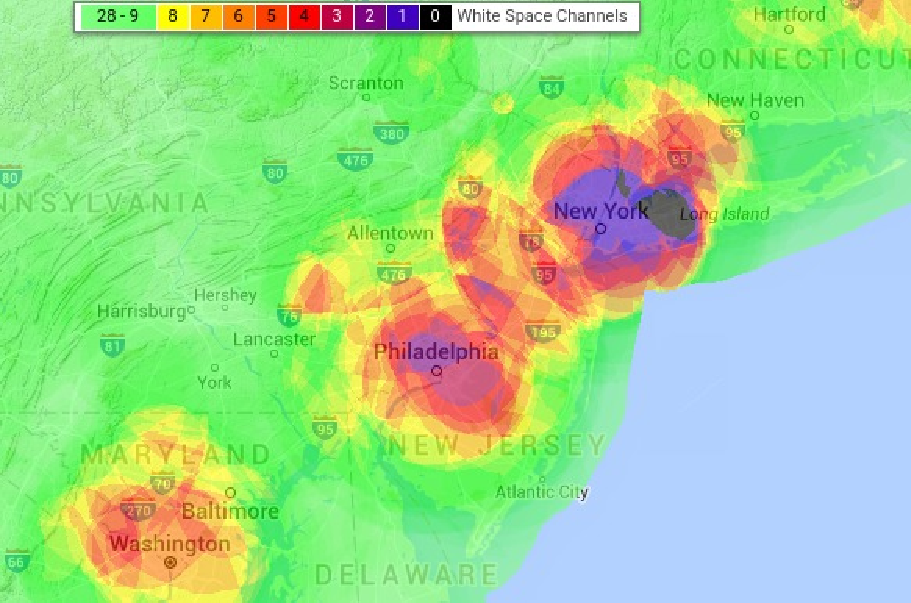
\includegraphics[width=0.9\linewidth]{TWWS_availability_east.pdf}
  \caption{Variability of available channels in a densely populated area. This figure is obtained from \cite{googleDatabase}}
\label{variability_TVWS}
\end{figure}

The white space devices are classified into two functional categories: 1) High power, stationary stations such a base stations , 2) lower power personal/portable devices, such as Wi-Fi network interface cards in laptops etc..
The fixed devices and some portable devices should access the WSDB to obtain the available spectrum and permitted transmission.
%
The fixed white space devices work as base stations and provides a backhaul for broadband client access.
These white space base stations (WBS) are the base stations in the IEEE 802.22 standard which is designed for wireless regional area networks.
As the fixed white space devices work with high transmission power, they are the major potential source of interference to the digital terrestrial TV receivers so that their transmission characteristics should be carefully decided by the TWDB.
According to regulations, the calculation engine within the WSDB translates the information of incumbent services and technical characteristics and location of the white space devices into a list of allowed frequencies and associated transmit powers for the white space devices~\cite{ECC236}.
WSDB's decisions on the transmission power are different with respect to different regulations.
ECC and Ofcom~\cite{ECC186, ECMA392} focus on the protection of the critical points from the harmful interference, and don't regulate the transmission power limitation. 
As to decision on the transmission power per ECC, as WBSs work in underlay manner and coexist with digital terrestrial TV receivers, the aggregate generated interference caused on the critical points on each channel should not exceed a threshold.
FCC initially restricts the maximum transmission power of the fixed devices to be 1 Watt and now relaxes the limitation to 4 Watt.
FCC doesn't impose restriction on the aggregated interference caused on primary TV receivers, hence there should be a limit on the number of operating WBSs when the WBSs in the IEEE 802.22 network are dense.
%
The existence of WSDB makes it a natural choice to adopt centralized solution for the channel allocation problem, \ie the WSDB not only provide the WBSs with the available channels and corresponding maximum powers, but also the channels to work on at a given time.
But where to make the channel allocation decision is not regulated, thus we will also provide distributed solutions.

In this paper, we focus on the co-existence issue of the WBSs and look into the channel allocation problem in TV white space with respect to ECC and FCC regulations respectively.
The main contributions of this work can be summarized as follows:
\begin{itemize} 
\item We devise both centralized and distributed schemes to make use of TVWS and improve the SINR on end users with respect to ECC and FCC rules respectively. To our knowledge, we are the first to focus on improving the SINR on the end users. 
\item We devise tailored distributed algorithms with respect to ECC and FCC regulations respectively. 
We formulate the channel allocation problem with different transmission power (ECC regulation) and the one with identical transmission power (FCC regulation) into congestion game respectively, and derive the distributed algorithms which converge to Nash Equilibrium. 
\item We solve the two centralized optimization problems and obtain the global optimal, both of them are binary and the optimization with respect to the FCC regulation is non-linear.
\item We outperform state of art in ECC regulation scenario.

\end{itemize}





%FCC issued a memorandum~\cite{FCC_2010_sedond_memorandumm,FCCdatabasae} in 2010, which removes the mandatory rigid sensing requirements, and prompts the usage of geolocations\footnote{Geolocation means both geographic location and terrain.}.
%FCC regulates a centralized database, which registers all the secondary users within one certain area, and decides on the available channels for them to use.
%The secondary users should access the database to obtain the list of available channels for the to use.
%The authors of ~\cite{SenseLess2011} validate this regulation and demonstrate the feasibility of only using geolocations and  propagation model.
%They adopt a central database which contains the geolocations of all TV stations.
%Then with sophisticated propagation model (Longley-Rice), the central database calculates the received signal strength index (RSSI) levels of TV UHF signals in a vast area.
%If RSSI on a channel is below a certain threshold on a location, TV service is regarded to be idle on that channel there and the secondary users there are allowed to use.
%The calculated results on channel availability is very close to the measurement results, which gives big impetus to the application of database mode in the exploration of TV white space.
%
%The FCC memorandum~\cite{FCC_2010_sedond_memorandumm,FCCdatabasae} and the work~\cite{SenseLess2011} initialize a new and easier way to utilize the TV white space, and the work~\cite{SenseLess2011} illustrates it is feasible to decide the RSSI level only with appropriate propagation model and geolocation.
%%Given the geolocation of the TV stations and secondary users, and appropriate propagation model, secondary users' maximum transmission power can be determined by the central entity according to the interference margin (maximum RSSI level from secondary users) on the TV receivers. 

%%ZZZZ modify the following paragraphs ZZZ
%In this paper, we investigate the efficient way to exploit the TV spectrum in a wireless regional area network which complies with IEEE 802.22 network.
%The secondary users are assumed to be cellular base stations and associated terminals, all of which work on TV white spectrum. 
%The base station is referred as WBS.
%%The corresponding secondary base stations are referred as white base stations (WBS). 
%Some cellular networks, \ie GSM or LTE network, work on licensed spectrum and emphasis on providing satisfactory services to their end terminals by choosing proper transmission channel and power. 
%As to cellular network working on TV white spectrum, they have to keep one eye on the primary users to make sure that TV service is not violated, which makes the problem of channel and power selection difficult.
%With the existence of central database, it is natural to utilize it as a central controller to assign channel and power usage for secondary users, but the secondary users may belong to different commercial groups and they may not contend with the assigned resource.
%%Besides, as the TV channels have different quality, \ie interference level, and permitted transmission power, it is difficult for the database to assign them to the 
%Hence, the spectrum sharing of the secondary users in IEEE 802.22 network should be decided in distributed manner and each secondary user takes care of its own interest, \ie to maximize its preferred utility.



The rest of the paper is organized as follows. 
We elucidate the system model in Section 2, afterwards related work is presented in Section 3. 
In Section 4, with respect to the regulation from ECC, we present the centralized optimization and game driven distributed scheme in terms of channel allocation.
In Section 5, with respect to FCC regulations, both centralized optimization and game driven distributed schemes are introduced.
Thereafter performance evaluation is presented in Section 6.
Finally, we conclude our work and point out directions of future research in Section 7.


\section{System Model and Problem Statement}
\label{SystemModel}
%According to the IEEE 802.22 standard, the primary systems considered in this chapter are digital TV (DTV) stations which use the TV spectrum legally. 
%TV stations provide service to passive TV receivers.
%The secondary users are IEEE 802.22 Wireless Regional Area Network base stations utilizing the TV spectrum with senseless mode~\cite{SenseLess2011}. 
%DTV's service should not be interfered by secondary systems. 

We consider an IEEE 802.22 compliant cellular network where the fixed white space devices work as base station and provide broadband access to their terminals.
The network is illustrated in Figure~\ref{sysmodel}.
We call the fixed white space devices which work as base stations as White space Base Stations (WBSs), they are located in one area which is surrounded by digital TV stations and receivers.
Several critical points are deployed in the vicinity of the digital TV receivers which are the most venerable to the interference caused by the white space devices.
WBSs work in underlay manner and coexist with the digital TV stations and receivers, the aggregate interference generated by WBSs should not exceed the threshold on each channel at each critical point.
%The aggregated interference on these critical points should below a certain threshold on all of the TVWS channels.
%
As to the WBSs, the out-of-band emission is regard as trivial, therefore, we only consider co-channel interference among the WBSs.
To simplify the analysis, we assume that each digital TV station as well as each WBS utilizes exactly one channel.\footnote{The assumption that one WBS only utilizes one channel is for convenience of analysis. In reality multiple channel usage (channel bonding) is requirement as one single TV channel's bandwidth is 6 MHz which is not adequate for a WBS to fulfill terminal demands. 
%We will relax this single channel usage assumption without hammering our scheme in the end of section \ref{sec_CA}.
}
%

As to the notations, the set of critical points is denoted as $\mathcal{K}$ and the set of WBSs is denoted as $\mathcal{N}$ where $|\mathcal{N}|=N$. 
The TVWS spectrum bands are denoted as set $\mathbb{C}$.
We represent the usage of channel for WBS $i$ with a binary vector $X_i^{|\mathbb{C}|\times 1}=\{x_i^1,\cdots, x_i^k,\cdots, x_i^{|\mathbb{C}|}\}\in \{0,1\}^{|\mathbb{C}|}$, where $k\in \mathbb{C}$ and binary variable $x_i^k$ denotes whether channel $k$ is used by user $i$. 
All the WBSs work with the channels approved by the WSDB, they operate with a channel from the approved ones after choosing it, thus we omit the time index in the channel usage.
As each node can only uses one channel, for $X_i$, there is $\sum_{k=1}^{|\mathbb{C}|}x_i^k=1$. 
The transmission power of WBS $i$ on channel $c$ is $P_i^c$.
$c(i)$ denotes the channel used by a WBS $i\in \mathcal{N}$. 

\begin{figure}[h!]
  \centering
  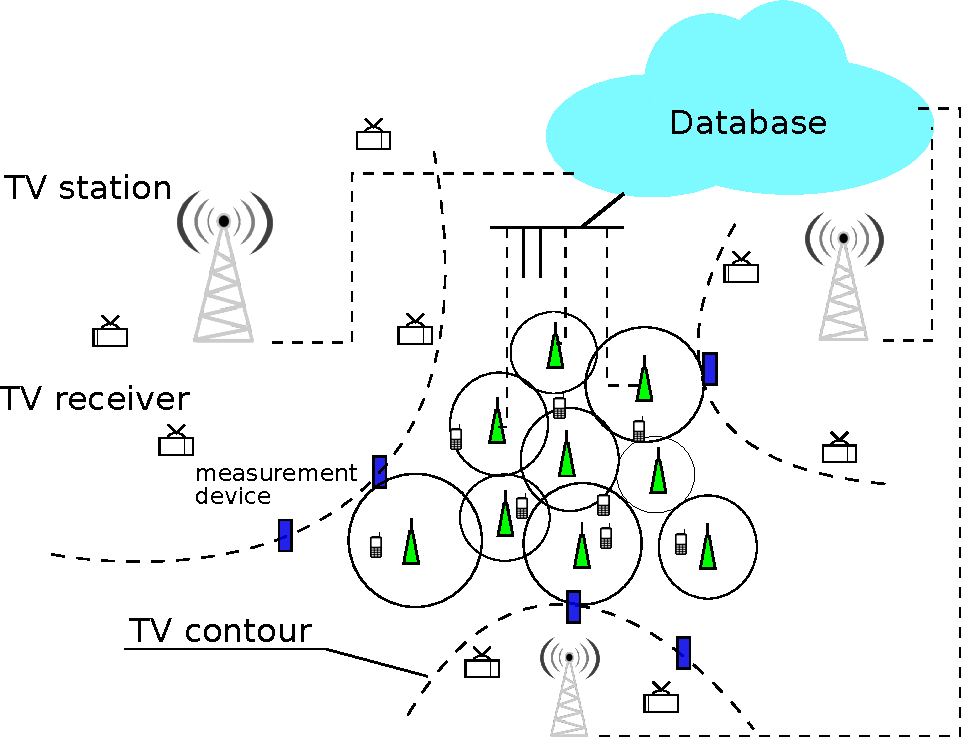
\includegraphics[width=0.9\linewidth]{systemmodel_working.pdf}
  \caption{System model: WBS cells and digital TV (DTV) systems}
\label{sysmodel}
\end{figure}
%In the rest of the chapter, we use WBS and secondary base station interchangeably. 
%There are interference measurement equipments deployed on the contours of TV service areas (as bold rectangles in Fig.~\ref{sysmodel}), which represent the worst located TV receivers in the TV service areas. 
%For these interference measurement devices, an interference threshold should not be violated by the noise generated by the secondary users.
%The deployment of the interference measurement devices is decided by the TV operators, which are usually along the contour of the area where TV receivers reside.
%Thus, the locations of interference measurement devices vary according to the concrete location, geographic terrain and possible deployment of secondary networks. 
%%For simplicity, we assume there is only one contour deployed for one TV area. % \todo{is contour 'clear' now?}.
%WBSs are deemed to be static.
%We assume the secondary base stations are not under the same operators, thus there is no scheduling mechanism available among WBSs.


For a terminal $m$ which is associated to WBS $i$, the attenuation between WBS $i$ and $m$ is denoted as $h_{im}$.
For the attenuation, we only take path loss and shadowing into account in the following.
The path loss is dependent on the distance between the corresponding equipment, e.g. $h_{im}=K \cdot d_{im}^{-\alpha}$, where $\alpha$ is the path loss exponent, $d_{im}$ is the distance between $i$ and $m$, while $K$ is a constant which models the reference loss over a single unit of distance.
Shadowing without fading is considered in our model.
$z_{im}$ models the zero-mean log-normally distributed shadow fading between $i$ and $m$, with the standard deviation $\sigma_{\text{SH}}$.
$N_0$ denotes the thermal noise power.
%
%The sum of all disturbing radio frequency effects (including interference) on terminal $m$ (we assume the working channel is $c$) is as following,
%\begin{equation}
%\label{interference}
%\begin{aligned}
%f_m^c=\sum_{\bar{i}} (P_{j}^c \cdot h_{jm} \cdot z_{jm}) +  N_0, \quad \quad j\in \mathcal{N}\setminus i, c(j) = c
%\end{aligned}
%\end{equation}
%where $P_{j}^c$ denotes the transmission power of interfering WBS $j$.
%Note that $z$ is dependent on the individual transmitter/receiver pair, but we omit the subscripts for simplicity. 
The SINR at end terminal $m$ is,
\begin{equation}
\label{SINR}
\begin{aligned}
\gamma_{m}  & = \frac{P_{i}^c \cdot h_{im}\cdot z_{im}} {f_m^c} & = \frac{P_{i}^c \cdot h_{im}\cdot z_{im}} {\sum (P_{j}^c \cdot h_{jm} \cdot z_{jm}) +  N_0}\\
					& &, \quad \quad j\in \mathcal{N}\setminus i, c(j) = c
\end{aligned}
\end{equation}
where $P_{j}^c$ denotes the transmission power of interfering WBS $j$.



%\subsection{Problem Statement}
In our model, we only assume the WBSs, which work with high transmission power, as the potential interfering unlicensed devices to the DTV service, meanwhile, WBSs are interested in providing broadband access to their associated terminals.
Our goal in this paper is to assign TVWS channel to each WBS so as to improve the signal to noise and interference ratio (SINR) of their associated end terminals, meanwhile complying with the prominent regulations \ie ECC and FCC.
The channels in $\mathbb{C}$ are assumed to be identical in terms of attenuation and shadowing on the same path.
%As to performance metric for the QoS provisioning, we choose the signal to noise and interference ratio (SINR) on the terminals.
A WBS's utility is a function of the SINR on all its end terminals, \ie the average SINR at all its terminals.

\subsection{QuasiSINR of WBS}
As to WBS's utility, it is not appropriate only to choose one terminal, as done in~\cite{spectrum_sharing_tvspace_2012}, or even multiple fixed terminals to represent the all the terminals in the same cell, because their locations could diverge greatly with the locations of the other terminals.
Thus, we propose a metric \textit{QuasiSINR} to represent WBS's performance in terms of SINR on its end terminals, which is independent on the actual locations of end terminals.


%We are interested in improving the SINR on the terminals of each cell by rendering WBSes to decide their channel and transmission power.
%The distribution of mobile terminals is varying and influenced by many factors, \ie the type of services provided to the terminals, the type of area and mobility of terminals.
%Thus when WBS decides its transmission parameter, it has to evaluate the SINR of all terminals.
%Furthermore, taking into consideration of terminals' SINR makes it very difficult to formulate WBS's preference on resources, \ie channel, power.
%Thus, we propose a simplified metric \textit{quasiSINR} for each WBS, which is independent on any terminals, and is able to  reflects the SINR on a circle around the WBS in a conservative manner.
%QuasiSINR can be easily adjusted by changing the radius of the circle so that the the circle goes through the majority of the terminal users.



%Instead of improving the SINR on each end users of WBSs, we propose a metric QuasiSINR to represent the services provided by WBSs to its end users.
%Then the utility of WBS becomes a function of the  and try to improve this metric.
%QuasiSINR is an indication of SINR that a WBS can provide to its terminals.
With an auxiliary circle centered at the discussed WBS, which is shown as dashed circle in Figure~\ref{quasiSINRfigure}, QuasiSINR is the ratio between the power of signal of interest on the circle and the summation of the strongest power from the interfering WBSs on the auxiliary circle.
%Assume WBS $i$ and all the other WBSs work on the same channel $c$, then co-channel interference are caused on its end users by all the other WBSs.
%The intersection of the auxiliary circle and the connecting line between WBS $i$ and one interfering WBS $j$, which is shown as red dot, is a reference point which corresponds to the interfering WBS $j$.
%There are multiple reference points on the auxiliary circle, which corresponds to the co-channel interfering WBSs respectively.
%The power of signal from $i$ on the auxiliary circle, the green dot, is the reference point for the power of signal of interest.
%The discussed WBS is denoted as $i$, and the rest WBSs are denoted as $j$, $j'$ and $j''$ respectively.
%We assume all the WBSs work on the channel $k$, this co-channel interference is caused on each WBS.
%An auxiliary dashed circle centering at WBS $i$ is shown, whose radius is $\delta$. 
%We can see both of the reference point of interference and the reference point for the power of signal of interest are largely decided by the radius of the auxiliary circle $\delta$.

\begin{figure}[h!]
  \centering
  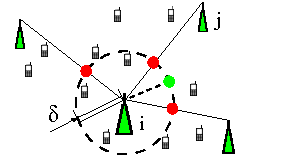
\includegraphics[width=0.6\linewidth]{quasiSINR2_2.pdf}
  \caption{Assuming the radius of the auxiliary circle is $\delta$ and all the WBSs work on the a channel, then QuasiSINR is a quotient where the divided is the WBS $i$'s power on the auxiliary circle (\ie the green pot), and the divisor is the summation of the interfering power on the red pots.}
\label{quasiSINRfigure}
\end{figure}


%The co-channel interference on the reference point of WBS $i$ from WBS $j$ is,
%\begin{equation}
%\label{quasiSINR_inf}
%\begin{aligned}
%f_{ji}^c = P_{j}^c\cdot h_{ji}\cdot z_{ji} = P_{j}^c\cdot (d_{ji}-\delta)^{-\alpha}\cdot z_{ji}
%\end{aligned}
%\end{equation}
%where $d_{ji}$ is the distance between WBS $i$ and $j$, while, $h_{ji}$ and $z_{ji}$ are the attenuation and shadowing from WBS $j$ to the relevant interference reference point.
%The sum of interference on WBS $i$' interference reference points is denoted as $f_{i}^c$.
%\begin{equation}
%\label{quasiSINR_infs}
%\begin{aligned}
%f_{i}^c = \sum_{j\in\mathcal{N}, c(j)= c} f_{ji}^c
%\end{aligned}
%\end{equation}
%
%The power of the signal of interest on auxiliary circle is expressed as,
%\begin{equation}
%\label{quasiSINR_1}
%\begin{aligned}
%\tilde{P_i}^c = P_i^c\cdot h_i\cdot z_i = P_i^c\cdot \delta^{-\alpha}\cdot z_i
%\end{aligned}
%\end{equation}
%where $h_i$ and $z_i$ are the attenuation and shadowing from $i$ to any point on the auxiliary circle.


The quasiSINR of WBS $i$ is denoted as $\gamma_{i}$, 
%\begin{equation}
%\label{quasiSINR}
%\begin{aligned}
% \gamma_{i} & = \frac{\tilde{P_i}^c}{f_i^c + N_0} \\
%&=\frac{P_{i}^c \cdot h_i \cdot z_i} {\sum_{\tiny\substack{j\neq i, j\in \mathcal{N}\\c(j)=c(i)}} (P_j^c \cdot h_{ji} \cdot z_{ji}) + N_0}\\
%&= \frac{P_{i}^c \cdot \delta^{-\alpha}\cdot z} {\sum_{\tiny\substack{j\neq i, j\in \mathcal{N}\\c(j)=c(i)}} (P_j^c \cdot (d_{ji}-\delta)^{-\alpha} \cdot z_{ji}) + N_0}
%\end{aligned}
%\end{equation}


\begin{equation}
\label{quasiSINR}
\begin{aligned}
 \gamma_{i} = &\frac{P_{i}^c \cdot h_{i\rightarrow \text{i's}\hspace{0.2em} \text{auxiliary circle}}\cdot z_{i\rightarrow \text{i's}\hspace{0.2em}\text{auxiliary circle}}} {\sum\limits_{\tiny\substack{j\neq i, j\in \mathcal{N}\\c(j)=c(i)}} (P_j^c \cdot h_{j\rightarrow \text{i's}\hspace{0.2em} \text{auxiliary circle}} \cdot z_{j\rightarrow \text{i's}\hspace{0.2em} \text{auxiliary circle}}) + N_0}\\
 = & \frac{P_{i}^c \cdot \delta^{-\alpha}\cdot z_{i\rightarrow \text{auxiliary circle}}} {\sum\limits_{\tiny\substack{j\neq i, j\in \mathcal{N}\\c(j)=c(i)}} (P_j^c \cdot (d_{ji}-\delta)^{-\alpha} \cdot z_{j\rightarrow \text{auxiliary circle}}) + N_0}
\end{aligned}
\end{equation}

In the following paper, when we talk about the channel and power allocation with respect to WBS, the notation $h_{ij}$ denotes the attenuation between WBS $i$ to the auxiliary circle of WBS $j$.
$h_{i}$ denotes the attenuation between WBS $i$ to its own auxiliary circle.
Then $\gamma_i$ becomes,
\begin{equation}
\label{quasiSINR_2}
\begin{aligned}
 \gamma_{i} = 
  \frac{P_{i}^c \cdot h_i\cdot z_i} {\sum\limits_{\tiny\substack{j\neq i, j\in \mathcal{N}\\c(j)=c(i)}} (P_j^c \cdot h_{ji} \cdot z_{ji}) + N_0}
\end{aligned}
\end{equation}
The abbreviations and notations used in this paper are summarized in Table~\ref{tab1}.
%
With auxiliary circle, the decision made by WBSs is independent on the distribution of the end terminals.
On the other hand, the radius of the auxiliary circle $\delta$ can be adapted to foster better service to the terminals in certain area, \ie a larger radius $\delta$ will take care of the SINR on the terminals reside far away and vice visa.
%When the terminals concentrate towards to the WBS, $\delta$ can be set smaller to better fit to the terminals' distribution.
%but it can also be set by operator according to the base station's situation, such as the distribution of end terminals, and the geography of the coverage of the base station. 
%For this terminal furthest away, we now construct a worst-case SINR which factors in all interference from neighboring secondary cells as if they were closest to the considered terminal. Hence, QuasiSINR is the ratio between the weakest signal of interest and the summation of the biggest (possible) interference from other co-channel WBSs. 

%any change of the transmit powers of co-channel interference source (i.e. other WBS working on channel $k$) will have always fixed impact to the quasiSINR of the WBS concerned, 
%As a result,  the concrete terminals are excluded from the channel and power allocation problem, which simplifies the problem to be discussed. 

%In the following part of this chapter, the notations are exclusively about the WBSs.

\begin{table}[h]
\caption{Notations}
\label{tab1}
\centering
\begin{tabular}{l p{5.5cm}}
\toprule
Abbr. & Description \\
Symbol & \\
\midrule
TVWS & TV white spaces\\
WSDB & white space database\\
WBS & white space base stations\\
$\gamma$ & QuasiSINR\\
$f_{ji}^c$  & The co-channel interference caused by WBS $j$ on the auxiliary circle of WBS $i$, $c$ is the working channel for both\\
$f_i^c$ & The sum of interference caused on the auxiliary circle of WBS $i$ \\
$p_i^c$		& The Tx power of WBS $i$ on channel $c$ on channel $c$\\
$P_i^c$		& The maximal permitted Tx power of WBS $i$ on channel $c$ (ECC solution)\\
$P_\mu, P_{\mathtt{op}}$		& The minimum and maximal permitted Tx power of WBS $i$ (FCC solution)\\
$h_{ij}$ & The attenuation between WBS $i$ to the auxiliary circle of WBS $j$.\\
$h_{i}$ & The attenuation between WBS $i$ to its won auxiliary circle.\\
$z_{ij}$ & The shadowing from WBS $i$ to the auxiliary circle of WBS $j$.\\
$z_{i}$ & in Section~\ref{whitecat}, the shadowing from WBS $i$ to its own auxiliary circle.\\
$\alpha_{ij}^k,\beta_{ij}^k$ & Binary auxiliary variables in the\\
$y_i, z_i$ & in Section~\ref{WhiteSussa}, optimization parameters.\\
$\text{cp}$ & Critical point\\
\bottomrule
\end{tabular}
\end{table}



In our model, WBSs access the WSDB and obtain the transmission parameters, \ie working channel, transmission power of the other WBSs, the attenuation characteristics between itself and all the other WBSs, and vice visa. 
WBSs calculate their QuasiSINRs with these information respectively.
%To obtain quasiSINR, one WBS doesn't need to measure the signal strength on the reference points which is needed in Formula~\ref{quasiSINR}, instead, it can can make use of the propagation model~\cite{Jaentti11} along with the operating parameters of all the other WBSs, which are stored in the central database to calculate the quasiSINR of any specific WBS.
%Besides, the channel usage of each WBS is also recorded in the data center.
%$h_{ij}$ and $z_{\bar{i}j}$, and also the transmission power of the interfering WBSs. 
%Thus when WBSes work in senseless mode, which can calculate the RSSI from one transmitter to an receiver with proper propagation model (e.g. Formula\ref{interference}\ref{SINR} can be calculated within database) with the geo-location and channel usage information. 
%A WBS also knows the interference it causes on the auxiliary circles of other co-channel WBSs via accessing the database.












\subsection{Problem Formulation}
\label{problemProposed}
Our goal is to minimize the sum of inverted quasiSINR $\sum_{i\in \mathcal{N}}\frac{1}{\gamma_{i}}$ with the WSDB's decisions on WBSs' transmission powers.
In order to ensure the fairness among WBSs,  we minimize the sum of inverted quasiSINR instead of maximizing the sum of quasiSINR of all WBSs.
%	\begin{equation}
%\label{problem}
%			\begin{aligned}
%			& {\text{Minimize}}
%			& & \sum_{i\in \mathcal{N}}\frac{1}{\gamma_{i}} \\
%			& \text{subject to}	
%			& & \sum_{k=1}^{|\mathbb{C}|}x_{ik}=1 \\
%			& & & P_{i,min}^c \leq P_i^c \leq P_{i,max}^c, c \in \mathbb{C}, i\in \mathcal{N}
%			\end{aligned}
%		\end{equation}
%		where $P_{i,min}^c$ and $P_{i,max}^c$ are the minimal and maximal transmission power of the transmitter of WBS $i$, where are restricted by the hardware configuration or capabilities.
%We assume $P_{i,min}^c$ and $P_{i,max}^c$ are identical for all WBSs and over all channels.

%XXX Please formalize the constraints, do not simply write 'one node, one channel'\todo{i'll do it!}
%where $\tilde{\gamma_{i}}$ is the QuasiSINR as defined in Equation~\ref{quasiSINR} XXX Always when you reference to a section, a figure, an equation or a table, mention the corresponding word in front of the reference - otherwise the reader does not know, should he reference to a section, an equation etc. - here I put in an 'Equation' for you but check this for the rest of the paper XXX. 
%\textcolor{blue}{TODO: In order to provide better service to its end users, WBS is motivated to choose the channel which either permits higher transmission power or experiences less interference, or the channel compromising the two factors according to Formula \ref{SINR}.
%Achieving optimal white spectrum allocation in a distributed style is the goal of this work, furthermore, this distributed solution should converge fast and lead to an efficient and stable solution.}


\section{Related Works}
\label{decomposition_relatedwork}



%In related works, the protection on primary users is taken care in the same time when channel and power selection are conducted.
%But according to the current regulations and standards, there exist no communication means between the secondary users and the primary users.
%Besides, when assuming such communication media is available and preventing primary users from being interfered during secondary users' power and channel allocation, the communication overhead between primary users and second users is considerable.

To exploit TVWS, authors in \cite{DySpAN10MeasuringWhitespaceCapacity, HessarTMC15, Deshmukh2015, Achtzehn12} have proposed different approaches for assessment of TVWS capacity under FCC and ECC regulations respectively.
Hessar et al.~\cite{ReAlloTVWS14DySPAN} aim to maximize the Shannon capacity of the network which complies with FCC rules.
The solution seeks the trade-off between the wide band and co-channel interference, both of which are brought by assigning multiple channels to WBSs.
But this scheme doesn't restrict the number of TVWSs and doesn't consider the harmful interference caused on the digital terrestrial TV receivers.
Yang et al.~\cite{yang2013WiFiWSTVCapacity} and Gopal et al.~\cite{gopalTCCN16} follow the rules of FCC, and propose throughput maximization of a CSMA/CA based WiFi like network in TVWS under aggregate interference.
Ying et al.~\cite{Ying2018DySPAN} look for the maximal set of white space devices which could access the spectrum, a heuristic scheme is proposed based on maximum weighted independent set in the graph which representing the secondary network.
This work doesn't consider the aggregate interference caused to the digital TV receivers.


%TODO-to modify
Omidvar et al. ~\cite{pimrc_2012} use potential game to propose a distributed joint power and channel allocation in cognitive radio network.
Although the scheme is not tailored for TVWS, protection on the primary users are also considered.
Potential game is adopted in work~\cite{Elias17} to mitigate the adjacent interference meanwhile bonding multiple channels.
In ~\cite{spectrum_sharing_tvspace_2012}, Chen et al. formulate the channel allocation problem in TV white space into a potential game where individual WBS's utility is to maximize the capacity of one static terminal.
%TODO: read the commented part.
%The execution of this scheme is formulated into an exact potential game. 
%For each base station, after several rounds of best responses in terms of channel and power level, Nash equilibrium is achieved.
%There are some flaws hindering the application of this scheme.
%Firstly, the paper doesn't provide means for base stations to obtain the needed information which is needed to calculate the utility function.
%Secondly, it is not clear how to calculate the punishment in the utility function, which indicates whether and how much the interference threshold on primary users is violated.
%Thirdly, the convergence speed of the scheme is not given, in fact, as the problem is formulated into a potential game, converge speed or the number of updates before convergence is a theoretic problem which is still unsolved.
%Last but not least, as the utility function and the potential in the game are designed as the sum of received and introduced interference, the desired signal power and the punishment, the minimization of this \textit{sum} does indicate meaningful  performance metrics, \ie SINR on terminals, or the total transmission power consumption.

\begin{comment}
\subsection{Problem Decomposition}
We obtain the maximal transmission power over each channel for every WBS before dealing with channel and power allocation, afterwards, the transmission power should not exceed this power mask.
The maximal transmission power over all channels for each WBS is obtained at the centralized database.
As the database has the global info of both the secondary network and primary network, the attenuation and shadowing between any two users are known \ie attenuation is based on propagation model and shadowing is obtained from measurement, the database is able to guarantee the service of primary users not be interfered when all the WBSs work on the same channel.
Meanwhile, as the secondary users belong to different groups of interest, the channel and power allocation should be done in distributed manner.
%By decomposing the problem into two subproblems, the protection on the primary users from harmful interferences is excluded out of the latter consideration on channel and power allocation.

%We propose a distributed workaround for the join power channel allocation problem, so that 
In summery, we solve the channel and power allocation in downlink communication in IEEE 802.22 network by solving three sequential subproblems:
\begin{itemize}
\item  Firstly, given a set of secondary WBSs and their geo-locations, the maximum permitted transmission power on each channel for each WBS is determined, so that the interference margin of primary users can not be exceeded no matter how WBSs utilize the spectrum and power resources.
In other words, the dynamics in the secondary network is transparent to the primary system. 
\item Secondly, once the maximum permitted transmission power is determined, WBSs choose their operating channels.
Note that this channel assignment problem is different from the works available in literature, where the transmission power is identical over different channels for different WBSs.
In this subproblem, the maximum permitted transmission power $p_i^c$ could be different for different channel $c\in \mathbb{C}$ and different WBS $i\in \mathcal{N}$.
\item Thirdly, working with the maximal permitted transmission power may not be the optimal in terms of power consumption and the SINR on terminals, thus distributed power adjustment is conducted and the working channel is unchanged.
\end{itemize}
%The first subproblem is a centralized approach, the following two problems are solved with distributed schemes.
%We name the our solution of channel and power allocation as \gls{DiCAPS} (Distributed Channel Allocation and Power Selection).
The solution to the channel allocation subproblem is named as \textit{whiteCat} (white space Channel allocation).

In the following, we introduce the related works of spectrum and power allocation problem in CRN, especially the works about the usage of TV white space.
we also introduce the works related with subproblems mentioned above.

%We discuss the detailed problems in the following two subsections in combination with related work in the respective area.
%XXX Di, how can it be possible that we set the maximum transmit power and let the secondaries choose their operating channel afterwards? Isn't this related to each other ? XXX  
%XXX Answer: I decide the maximal transmission power in a very conservation way: let all of the WBSs work on the same channel and decide the max power. This need strong argument XXX

%In this paper we contribute by addressing this problem from two complementary directions. On the one hand, we study a convex formulation for setting the maximum transmit power at a set of secondary users given different interference margins for primary users. This scheme assumes a central controller to be in place which has geo-information and sufficiently detailed radio maps to characterize the path loss. We show that this convex formulation provides superior performance compared to linear problem formulations proposed in related work. Furthermore, we address the problem of assigning channels to WBS. Here, apart from the resulting cell performance, we also consider convergence of the assignment scheme as well as power consumption as important metrics. We propose a distributed scheme which interacts with a data base to get to know the channel choices of neighboring base stations, the interference relationships as predicted by radio maps as well as the maximal transmit powers. Formulated into a congestion game, the proposed schemes converges fast and provides superior performance in terms of cell performance and power consumption. 


\subsection{Resource Allocation in CRN}

We will emphasis more on the distributed solutions, but in order to give readers a full picture of the solutions as to resource allocation in CRN, we will also introduce the related works on centralized solutions.

Centralized solutions usually solve the formulated constrained optimization problems at a centralized unit.
In \cite{downlink-centralized-08-TWC}, the objective is to increase the number of supported terminals whose SINRs are above a threshold, and the constrains are to refrain the interference at the primary users within a certain margin.
Work \cite{joint_power_channel_linkpair_08ICT} minimizes the transmission power and meanwhile makes sure the SINR of terminal is above a threshold, but this work fails to consider the protection of primary users.
A heuristic algorithm is proposed in \cite{centralized_80222_sharing_ifip2011}, which considers the channel availability and transmission demand of each WBS.
The aforementioned two schemes don't consider varying the transmission power.
% xxxx important paper
%A centralized scheme is proposed in \cite{nashbargaining_2012jsac} for joint channel and power allocation among end terminals in OFDM cognitive radio network. 

There is a large variety of distributed solutions.
In order to avoid or to alleviate co-channel interference between cells, and to allow arbitrary number of cells to work in IEEE 802.22 network, \cite{Inter-Network_Spectrum_Sharing_80222_08} proposes distributed inter-network spectrum sharing scheme, where contention decisions are made in a distributed way and the winner cells can use the shared channels.
But this work doesn't consider the role of transmission power in the co-channel interference.
An distributed power allocation (single channel) scheme based on learning for secondary networks is given in \cite{aggregatedInf_Galindo_crowncom09}, where penalty function involving the interference threshold on primary systems is used.
%
\cite{HoangPowerChannel2010} discusses power control and channel assignment in both down-link and up-link communication in cellular network. 
Although the solution is distributed, primary users are required to cooperate with secondary base station in a learning process to decide the transmission power, in addition, there is only one secondary base station considered whereas we need to cope with the multiple cells in our problem.
%
Joint channel-power selection for multiple transmission links (pairs) is investigated in \cite{wuinfocom09}. 
The authors decompose the Lagrangian dual of the problem, then propose a distributed scheme based on the dual parameters. 
The scheme converges into pure Nash equilibrium, but in order to facilitate this scheme, monitors are required to watch interference from secondary users, moreover, monitors have to be equipped computational ability and interact with secondary users in the whole process of convergence.
%

As introduced in Chapter~\ref{INTRODUCTION}, game theory is a powerful tool in designing distributed algorithms.
A distributed joint power and channel allocation is proposed in~\cite{pimrc_2012}, each base station chooses optimal power level and channel to optimize its utility, which results in induced received interference and caused interference on primary users. 
The execution of this scheme is formulated into an exact potential game. 
For each base station, after several rounds of best responses in terms of channel and power level, Nash equilibrium is achieved.
There are some flaws hindering the application of this scheme.
Firstly, the paper doesn't provide means for base stations to obtain the needed information which is needed to calculate the utility function.
Secondly, it is not clear how to calculate the punishment in the utility function, which indicates whether and how much the interference threshold on primary users is violated.
Thirdly, the convergence speed of the scheme is not given, in fact, as the problem is formulated into a potential game, converge speed or the number of updates before convergence is a theoretic problem which is still unsolved.
Last but not least, as the utility function and the potential in the game are designed as the sum of received and introduced interference, the desired signal power and the punishment, the minimization of this \textit{sum} does indicate meaningful  performance metrics, \ie SINR on terminals, or the total transmission power consumption.
In~\cite{spectrum_sharing_tvspace_2012}, Chen et al. investigate the channel allocation problem in the scenario of TV white space.
The channel allocation problem is formulated into a potential game, individual WBS's utility is to maximize the capacity of one single static terminal.
%
Potential game is also adopted in work~\cite{tvws_paper_networking2015} to design algorithms, which mitigates the adjacent interference.
%
\cite{powerChannelAllocation_2015_shapley} adopts cooperation game to research the coexistence of femtocells.
Each femtocell negotiates with neighbouring fremcells, and they form temporary coalition, but the goal of this solution is to allocate resource block in terms of time and transmission power.
\cite{joint_power_channel_linkpair_08ICT} proposes both centralized and decentralized solutions.
Two distributed schemes are proposed, joint channel and power allocation is formulated into a weighted potential game, as an alternative workaround, the problem is solved in two sequential phases.

%
Distributed algorithm based on Learning is proposed in \cite{cogCE_huang} for LTE to allocate the the resource block in down link, which leads to correlated equilibrium, but slow converge hinters its application.
%



\subsection*{Utilization of TV White Space}
Here we introduce the solutions proposed on the utilization of TV white space, which includes regulations, proposed standards and recent research advances.
In accordance with the regulations of FCC, there are some prototype applications proposed in both cellular network~\cite{tvwhite_lte2011, multicell_geo_dyspan11} and WiFi-like network~\cite{whitefi09}.
The secondary users access a centralized data base to know the allowed channels and transmission power.
%
Standardization bodies are also working on TVWS utilization, including IEEE 802.22~\cite{802.22} for Wireless Regional Area Networks (WRAN), IEEE 802.11af~\cite{802.11af} for WLAN, IEEE 802.15.4m~\cite{802.15.4m} for 802.15.4 wireless networks in TVWS and 802.19.1~\cite{802.19} for coexistence methods among local and Metropolitan Area Networks (MAN).

%\cite{HoangPowerChannel2010} proposes a distributed solution for power control and channel assignment in both down-link and up-link communication in a WRAN, but the investigated secondary network is composed with only one base station and multiple terminals.

%% related work!!!
Scientific research on utilization of TVWS goes on in parallel with the regulatory agencies.
Feng et al.~\cite{hybridPricing_tvspace_2014} investigate the business model of TV spectrum utilization in database involved network structure, emphasis on the price policy of the channels approved by FCC.
Spectrum sharing in TVWS is formulated as a series of optimization problems. 
The guarantee that TV receivers should not be affected by the aggregate interferences form TVBDs is one constraint.
The objective can be maximizing TVBD's downlink transmission power~\cite{multipleIntf_pimrc11}, uplink transmission power~\cite{uplink_power_tvws13}, or best geographic distribution of TVBDs~\cite{withinTVcoverage_PIMRC13}.
A series of works~\cite{game_CA_association_ICDCS12,SA_CA_TVWS_2012crowncom, 802.22co-existence09, 802.22game_08globecom,self-coexistenceWRAN2010infocom} emphasise on interference mitigation among TVBDs via spectrum allocation.
Vehicular networks operating with TVWS assisted by TV database and cooperative sensing is discussed in~\cite{tvws_vtc13}.
Work~\cite{increaseTVWS12} steps further from the database paradigm and makes efforts to utilize the \textit{grey space}, where white space device is allowed to operate even within the TV service area.

%After each update, WBS needs to access the data base to retrieve the current channel usage, then they can calculate xxx.




%Secondary network should not interfere TV receivers, thus regulation on transmission power is necessary.
%\cite{Chen_PowerControl,SenhuaHuang10,Zhu09} propose schemes for secondary users to decide the transmission power with sensing technology, one prime consideration of schemes is obviating interfering incumbent primary users. A distributed scheme to adjust power based on learning is proposed in \cite{aggregatedInf_Galindo_crowncom09} for each WBS, where a penalty function involving the interference threshold is used. This scheme needs many steps to converge, and there is no interference margin for network dynamics.
%Solving the joint problem of power and channel allocation in a distributed manner is challenging.
  
To protect the TV receivers from harmful interference, the aggregate interference caused by WBSs at the contours of TV receivers should not exceed the interference margin.
Work \cite{maximum_power_TVWS_dyspan_2011} proposes detailed calculations which a geolocation database performs in order to derive location-specific maximum permitted EIRP levels for white space devices which operate in digital terrestrial TV bands.
\cite{multipleIntf_pimrc11} considers the maximum permitted transmission power for the network which complies with IEEE 802.22 standard. 
The standard requires a centralized database to store the available channels for each secondary base station, thus centralized scheme can be conducted there after trivial modification.
The sufficient condition for the TV receivers not be interfered in the context of TV white space is formulated into a centralized linear programming program (LP) in~\cite{multipleIntf_pimrc11}.
The objective function is to maximize the summation of all secondary base stations' transmission power, and the constraints are formed to satisfy the sufficient condition for every interference measuring device for the TV receivers. 
However, this approach doesn't take the channel assignment problem into account.
%XXX This discussion of the related work is a bit confusing. The problem is that it is no clear per discussed paper what the shortcoming of the approach is. I.e. you describe the approaches but you do not help the reader why this approach is not contributing to the goal defined in the first sentence. Try to reformulate this section more precisely expressing what is the problem with the corresponding approach XXX.

\end{comment}

With the doctrine of not interfering the primary TV services and regulations imposed by institutes, the problem we solve in this paper is different from the channel allocation problems discussed in the domain of cognitive radio networks.
But we think a brief review in terms of the channel allocation techniques in CRN is necessary.
%
%Channel assignment problem can be converted into colouring problem thus is NP hard~\cite{Hyacinth}. 
%Authors of~\cite{Ko_DistributedCA} propose best response to improve the transmitters' utilities, but best response process can only converge when the transmission powers are identical and path loss is symmetric.
With identical transmission power and symetric path attenuation, Nie et al.~\cite{CApotentialLearning_05dyspan} formulate channel assignment problem in ad-hoc cognitive radio network into a potential game which leads to pure NE, the authors~\cite{CA_Felegyhazi_07infocom, Wu_GOP_CA_08infocom} propose algorithms which converge to pure Nash equilibrium (NE) and strongly dominate strategy equilibrium respectively. 
Simulated annealing is applied to mitigate co-channel interferences in~\cite{SA_CA_TVWS_2012crowncom}.
For the same purpose, no-regret learning~\cite{qlearning_huang, hart00correlatedeq} is exploit to optimize the choice on channel.
in~\cite{hart00correlatedeq}, each WBS maps the probability of choosing each strategy to a certain proportion of the regret which the WBS may have if it doesn't choose that strategy, and the WBS choose the strategy with the biggest probability.  
WBSs update such mapping dynamically and this approach converges to correlated equilibrium. 

%As to our knowledge, there is no work dealing with channel allocation problem where transmission power is different.
%XXX So here we have the same problem as above: Only for the first two papers you say explicitly what problems come up with them - for the rest you simply mention them and their approach. Here we really need a much more clearer formulation of the shortcomings - why are they failing to be a solution to our problem ? Furthermore, there seem to be quite a lot of work in game theory and power control in secondary networks - how do they relate to our work? XXX

%Channel allocation facilitates CRN to improve throughput~\cite{channelAllocation_throughput_12wcnc}, or cooperatively relay~\cite{channelAllocation_relay_2010ICASSP} and so on.
%This thesis emphasises on co-channel interference mitigation with distributed channel allocation. 



%In this work we concern the best possible quality-of-service provisioning by allocating channels on which fixed transmission power is used.
%In this paper we try to improve the SINR on secondary end terminals through WBSs' power-channel strategy. To facilitate analysis and proposition of solution, we propose a metric \textit{QuasiSINR} for each secondary base station to represent the SINR of the terminals in the coverage of that base station.


%\todo{todo:}
%\begin{itemize}
%\item what is the reason to design a distributed scheme for this problem.
%\begin{itemize}
%\item complexity (to w)
%\item overhead
%\item WBSs belong to different commercial organization (we actually propose a spectrum sharing paradigm)
%\end{itemize}
%
%\item argument 1: why is the utility used in the algorithm, in other words, what is the reason to chose it and what is the relation between it and the SINR on end users.
%
%\end{itemize}

\section{Channel and Power Allocation Scheme complying with ECC Rules}

In this section we will discuss the channel and power allocation problem complying with the rules regulated by ECC.
Given all the other WBSs' selection on channel and transmission power, a WBS is interested in choosing the channel which brings it the best performance, \ie the data rate of its end users.
A WBS prefers to choose the channel which experiences the minimum interference, while simultaneously the transmission power can be set as high as possible, so as to obtain better SINR at associated terminals and and generally increase coverage. \cite{wuinfocom09, HoangPowerChannel2010}. 
Nevertheless, high transmission power causes significant co-channel interference to other secondary users operating on the same channel. 
Hence, a secondary cell has to balance its transmission power and the caused interference on other cells while simultaneously choosing a working channel that decreases the interference its terminals are exposed to.
In the following subsections, we firstly present the decision on the maximum permitted transmission power on each channel for each WBS, then present how do the WBSs make use of these powers in both centralized and distributed manner respectively.
\subsection{The Maximum Permitted Transmission Power}
\label{powermap}

We adopt the interference model and the optimization methodology from the work of \cite{multipleIntf_pimrc11} to plan the maximum transmission power on each channel for WBSs.
%
For WBS $i\in \mathcal{N}$, the maximum transmission power allowed on channel $c\in \mathbb{C}$ is denoted as $P_i^c$. 
As to each channel $c$, the generated interference on each interference measuring device should be within a predefined interference margin $I$.
The interference margin in a slow fading environment is decided according to~\cite{aggregate_interference_shadow_fading_2010}.
To address this fairness issue, we maximize the sum of the logarithmic value of every WBS's transmission power, and formulate the problem into a convex optimization problem.
	\begin{equation}
		\label{cvx}
		\begin{aligned}
		& {\text{Maximize}}
		& & \sum_{i\in \mathcal{N}} \log P^c_i \\
		& \text{subject to}
		& & \sum_{i\in \mathcal{N}} (P^c_i \cdot h_{i,\text{cp}}\cdot z) < I, \forall\text{cp} \in \mathcal{K}
		\end{aligned}
	\end{equation}
This optimization is conducted in WSDB for each channel $c\in \mathbb{C}$, and the calculated maximum permitted transmission powers are used by the WBSs afterwards.
The interference threshold on the critical points will not be exceeded even when all the WBSs work on one same channel.

%there are multiple channels available and WBSs are free to choose their preferred channels, the aggregate interference on one channel will be smaller than that when all WBSs work on that channel. 
%When the WBSs work on different channels, there will be a margin for network dynamics such as new WBS starting to work or increased interference on TV contour due to the variance of broadcast path condition. 
%XXX As mentioned above, it is not clear which impact the relationship between maximum transmit power planning and channel selection has XXX.


\subsection{Centralized Optimization for Channel Allocation}
\label{03_centralized_ca}

%We formulate the channel allocation problem into a binary quadratic programming problem.  
%Let $X_i = \{x_i^1,\cdots, x_i^k,\cdots, x_i^{|\mathbb{C}|}\}$ denote the vector of channel usage, there is $|X_i| = |\mathbb{C}|$ and binary element $x_i^k$ represent whether WBS $i$ occupies channel $k$.
Given two WBSs $i$ and $j$, the co-channel interfering relationship is decided as,
\begin{equation}
\begin{split}
X_i^TX_j = \sum\limits_{k=1}^{|\mathbb{C}|}x_i^k\cdot x_j^k = 
\left\{ \begin{array}{ll}
1 & \mbox{if $c(i)=c(j)$} \\
0 & \mbox{if $c(i)\neq c(j)$} 
\end{array}
\right.
\end{split}
\end{equation}

%$c(i)$ means the working channel which is chosen by WBS $i$.
The transmission power levels on all channels for WBS $i$ are denoted by a constant vector $\vec{P}_i = \{P_i^1,\cdots, P_i^k,\cdots, P_i^{|\mathbb{C}|}\}$. 
The transmission power adopted by WBS $i$ is $\vec{P}_i^TX_i = \sum\limits_{k=1}^{|\mathbb{C}|}P_{i}^k\cdot x_i^k$.


The problem in Section~\ref{problemProposed} is formulated as a general purpose nonlinear optimization,
	\begin{equation}
\label{03_centralized_ca_Optimization}
		\begin{aligned}
		& \underset{}{\text{minimize}}
		& & \sum\limits^{n}_{i=1} \frac{\sum\limits_{j\in\mathcal{N}, j\neq i}\vec{P}_j^TX_j(X_j^TX_i)h_{ji}z_{ji} + N_0}{\vec{P}^TX_ih_iz_i}\\
		& \text{subject to}
		& & \sum\limits_{k=1}^{|\mathbb{C}|}x_i^k=1, x_i^k\in X_i\in \{0,1\}^{|\mathbb{C}|}\\
		\end{aligned}
	\end{equation}
Problem \ref{03_centralized_ca_Optimization} is a non-linear problem with binary variables, but it can be transformed into a quadratic programming problem as follows,
	\begin{equation}
\label{QLP_2}
			\begin{aligned}
			\underset{}{\text{minimize}}
			& \sum\limits^{n}_{i=1} ( \sum\limits_{j\in\mathcal{N}, j\neq i}\sum\limits_{k\in\mathbb{C}} \frac{P_j^k\cdot h_{ji}\cdot z_{ji}}{P_i^k\cdot h_i\cdot z_i}\cdot  x_j^k\cdot x_i^k  \\
			& + \sum\limits_{k\in\mathbb{C}} \frac{N_0}{P_i^k\cdot h_i\cdot z_i}\cdot x_i^k)\\
			\text{subject to} 
			& \sum\limits_{k=1}^{|\mathbb{C}|}x_i^k=1, x_i^k\in X_i\in \{0,1\}^{|\mathbb{C}|}\\
			\end{aligned}
		\end{equation}

The reformulation is available in Appendix in our previous work \cite{Li2012DistributedTS}.
We use GUROBI~\cite{gurobi} which is a state of art non-linear problem solver to solve the problem, which employs Branch-And-Reduce method to get the global optimum for the problem. % We use the results obtained by solving this QLP problem as one reference in the coming section. 
%The result of this centralized channel assignment will be evaluated in the simulation section with other schemes. 



\subsection{Distributed White Space Channel Allocation (WhiteCat)}
\label{whitecat}
In this section a distributed scheme for WBSs to allocate channels meanwhile complying with ECC regulation is proposed, which is named as \underline{white} space \underline{c}hannel \underline{a}llocation \underline{t}echnology (WhiteCat). 

\subsubsection{Algorithm and Protocol}
WhiteCat adopts the best response process, where each WBS (referred as $i$) chooses the channel which brings the largest utility $u_i$, as shown in Formula~\ref{utility}, as the response of other WBSs' choices on channels.
%and the sum of all WBSs' utilities is minimized after finite times of updates even the interaction between WBSs are asymmetric. The utility is as follows,
WhiteCat is depicted by Algorithm \ref{whitecatalgo}.

\begin{equation}
\label{utility}
u_i =\dfrac{\sum\limits_{\tiny\substack{j\in \mathcal{N}, j\ne i,\\ c(\sigma_j)=c(\sigma_i)}}f_{ji}}{2\cdot \tilde{P_i}} + \dfrac{1}{2}\sum_{\tiny\substack{j\in \mathcal{N}, j\ne i,\\ c(\sigma_j)=c(\sigma_i)}}\dfrac{f_{ij}}{\tilde{P_j}} + \sum_{\tiny\substack{\mathcal{S}:i,j\in \mathcal{S},\\ c(\sigma_j)=c(\sigma_i)}}\dfrac{N_0}{C\cdot \tilde{P_i}}\\
\end{equation}

where $\tilde{P_i} = P_i\cdot h_i\cdot z_i$, similarly $\tilde{P_j} = P_j\cdot h_j\cdot z_j$.
Overlooking the constant coefficient 2, the first item of $u_i$ is the inverted QuasiSINR of station $i$. 
To minimize the first item, WBS $i$ needs to choose a channel either permits higher transmission power or experiences less interference, whereas the higher power increases the second item which is a part of inverted QuasiSINR of other co-channel WBSs. 
Hence, the cost function presents a reasonable compromise between the QuasiSINR of one WBS and others.

When WBS only emphasizes on its own utility (e.g. the first part of Formula~\ref{utility}), the best response process doesn't always converge and we have following theorem:
\begin{theorem}
\label{noconvergence}
\emph{With non-identical transmission power, if every WBS updates its channel based on Algorithm \ref{whitecatalgo} with utility based on its own interests, \ie the first part of Formula~\ref{utility}, the process doesn't always converge.}
\end{theorem}
The proof is in Appendix 1 in~\cite{Li2012DistributedTS}.


\begin{algorithm}[h]
\caption{Spectrum selection by WBS $i$}          % give the algorithm a caption
\label{whitecatalgo} 
\DontPrintSemicolon
\SetAlgoLined
\KwIn{the distance, path lose and shadowing parameter between WBS $i$ to WBS $j\in \mathcal{N}\setminus i$;\\  radius of auxiliary circle, noise $N_0$, total number of WBSs $N$;\\ for $j\in \mathcal{N}\setminus i$, the maximal transmission power $P_j^c, c\in \mathbb{C}$ and the working channel $c(j)$.
}
%\KwOut{a channel }

	\For{$c\in \mathbb{C}\setminus c(i)$}{
	 calculate $u_i(c)$ based on Formula \ref{utility}
	 \eIf{$u_i(c)<u_i(c(i))$}{
	 	$c(i)\leftarrow c$
	 }
	 {keep $c(i)$ unchanged}
	}
	
Notify database of its channel usage, which further notifies the other WBSs

\end{algorithm}

%Some parameters needed to calculate the utility are identical for all WBSs, such as quasi distance $e$, the total number of WBSs $N$, number of channels $C$, attenuation factor $\alpha$, standard deviation $\sigma_{WBS}$ in flat shadowing and noise $N_0$, albeit 

%Similar with~\cite{SenseLess2011}, we let every WBS store the location information and maximal power map of all other WBSs, \ie $P_i^c, i\in\mathcal{N}, c\in\mathbb{C}$, and each WBS retrieves information about channel usage of other WBSs from centralized base station.

WBSs calculate $u_i$ with the information retrieved from WSDB.
After executing Algorithm \ref{whitecatalgo}, WBSs report to WSDB about their chosen channels if they are updated.
As the locations of WBSs and TV stations, along with the transmission channel and power of TV stations are usually static (entries of TV station change averagely once in 2 days\cite{SenseLess2011}), except for the channel usage in the network, the change of the other data stored in WBS is infrequent. 
We refer \cite{CApotentialLearning_05dyspan} to decide WBSs' sequence to update their channels.
\cite{CApotentialLearning_05dyspan} proposes a method which is akin to the random access mechanism of CSMA/DA, where the access for broadcast medium is changed to get access to the centralized center to retrieve the current channel usage and update its new channel. 
All WBSs are able to access the database in one round (with random or predetermined sequence). 
%As WBSs are connected with database, the control messages needed to decide the sequence will not become a burden. 
Update of channels can happen in several scenarios, \ie in boot phase, or when the SINR on end users falling below a threshold, or a fixed time duration coming to end, or new WBSs joining in the network. 


\subsubsection{Analysis in Game Theoretical Framework}
\label{game}
In this section, We give the proof on whiteCat's convergence in the framework of congestion game theory.
Formulating a spectrum sharing problem into a congestion game and the concept of \textit{virtual resources} are firstly proposed in \cite{allerton08_liu}.
This work reversely engineers the distributed channel allocation schemes proposed in \cite{babadi_08, Ko_DistributedCA}, \ie unifies the algorithms with congestion game.
But the problem analysed in~\cite{allerton08_liu} assume the transmission power is identical, which is a major difference from the channel allocation problem discussed here. 

%\subsubsection{Congestion Game}
%A congestion game \cite{Rosenthal}\cite{Voecking06congestiongames} can be expressed by a tuple $\lambda=(\mathcal{N},\mathcal{R},(\sum_i)_{i \in \mathcal{N}},(g_r)_{r\in \mathcal{R}})$, where $\mathcal{N}=\left\{1,\ldots,N\right\}$ denotes the set of players (each each is labeled with a unique index number), $\mathcal{R}=\left\{1,\ldots,m\right\}$ the set of resources, $\Sigma_{i\in\mathcal{N}} \subseteq 2^{\mathcal{R}}$ is the strategy space of player $i$. Under strategy profile $\sigma=(\sigma_1,\sigma_2,\cdots \sigma_N)$, player $i$ chooses strategy $\sigma_i\in \Sigma_i$, and the total number of users using resource $r$ is $n_r(\sigma)=|\{i\mid r\in \sigma_i\}|$. The cost $g_r: \mathbb{N}\rightarrow \mathbb{Z}$ is a function of the number of users for resource $r$, $g_r^i=\sum_{r\in \sigma_i} g_r(n_r(\sigma))$. In our paper, $g_r^i$ is referred as \textit{congestion} and is Monotonic.
%
%Rosenthal's potential function $\phi:\sigma_1\times\sigma_2\times\cdots\times\sigma_n\rightarrow Z$ is defined as:
%\begin{equation}
%\label{4}
%\begin{split}
%G(\sigma) 
%& =\sum\limits^{}_{r\in \mathcal{R}} \sum\limits^{n_r(\sigma)}_{i=1} g_r(i)\\
%& =\sum\limits_{i\in \mathcal{N}} \sum\limits^{}_{r\in \sigma_i} g_r(n_r^i(\sigma))\\
%\end{split}
%\end{equation}
%$n_r^i(\sigma)$ means the number of players using resource $r$ and \textit{their indices are smaller than or equal to $i$}. Note that the potential is \textit{not} the sum of congestions experienced by every user. The change of the potential caused by one player's unilateral move from $\sigma$ to $\sigma'$ is equivalent to the change of gain (or loss) of that player.
%\begin{equation}
%\label{5}
%\varDelta G(\sigma_i \rightarrow \sigma_i') = g^i(\sigma_i',\sigma_{-i}) - g^i(\sigma_i,\sigma_{-i})
%\end{equation}
%$\sigma_{-i}$ is the strategy profile for all players except for $i$.
%As every congestion game is a potential game, and the total potential is finite, thus the number of improvements is upper-bounded by $2\cdot\sum\limits^{}_{r\in \mathcal{R}} \sum\limits^{n_r(\sigma)}_{i=1} g_r(i)$ \cite{Voecking06congestiongames}.
%
%
%We have introduced congestion game in Chapter~\ref{background}, thus we only recap the essence of congestion game here.
In congestion game, each player acts selfishly and aims at choosing strategy $\sigma_i\in \Sigma_i$ to minimize their individual cost.
The gain (loss) caused by any player's unilateral move is exactly the same as the gain (loss) in the potential, which may be viewed as a global objective function.
For problems where the potential of the problem is the same with the summation of the cost of all users, the cost function can be used as a utility function directly.
This equivalence doesn't exist in our problem, but by carefully choosing the cost function for players, we can make sure that the change of individuals' cost is in the same direction with that of the global utility.



\subsubsection{From WhiteCat to Congestion Game}
\label{gameforproblem}
We utilize the conception of virtual resource which is firstly introduced in \cite{allerton08_liu}. 
Virtual resource is a triplet $\{i, j, c\}$, where $i,j$ are two WBSs and $c\in \mathbb{C}$ is one channel.
This piece of resource is regarded used by $i$ when both $i$ and $j$ use channel $c$, otherwise, $\{i, j, c\}$ is not used by any WBS.

In the following, we list the element of the congestion game which emulates Algorithm~\ref{whitecatalgo}.
In this section, player and base station are used interchangeably.

\begin{itemize}
\item Player $i$' strategy space is $\Sigma_i=\{(i,j,c), j\in \mathcal{N}, j\ne i, c(\sigma_j)=c, c=1,2,\cdots,N\}$, and $i$ has $C$ admissible strategies, one strategy related with channel $c\in\mathbb{C}$ is described by the set of virtual resources it uses: $\sigma_i=\{(i,j,c), j\in \mathcal{N}, j\ne i, c(\sigma_j)=c\}$, note that virtual resource $(i,j,c)\neq(j,i,c)$.

\item Under the strategy profile $\sigma=(\sigma_1, \sigma_2, \cdots \sigma_N)$, player $i$ obtains a total cost of 

	\begin{equation}
\label{6}
		\begin{split}
		g^i(\sigma)= \sum\limits^{}_{\tiny\substack{j\in \mathcal{N},j\neq i,\\ c=c(\sigma_i)=c(\sigma_j)}} &(g_{(i,j,c)}(n_{(i,j,c)}(\sigma))\\&+g_{(j,i,c)}(n_{(j,i,c)}(\sigma))
		\end{split}
		\end{equation}
\end{itemize}

The transmission power over all channels of player $i$ is $\{p_i^1, p_i^2,\cdots, p_i^{|\mathbb{C}|}\}$.
%According to our system model, interfere xxxxxx
%Path loss is assumed reciprocal: $h_{ij}=h_{ji}$, but nor is the flat fading $z$. To keep the formula clear in the following part, we denote $\tilde{f_{ij}}= P_i\cdot h_{ij}\cdot z$, $\tilde{f_{ji}}= P_j\cdot h_{ij}\cdot z$, $\tilde{P_i}=h_{iQ}$ for $i\in \mathcal{N}$, where $h_{ji}=h_{ij}=(d_{ji}-e)^{-\alpha}, h_{ii}=h_{jj}=e^{-\alpha}$, $d_{ji}$ is the distance between base station $i$ and $j$, and $\delta$ is the quasi distance introduced in section \ref{SystemModel}. $N_0$ is noise which is identical for any channel and any WBS. 
We define the cost function for virtual recourses $(i,j,c)$ as follows,
\begin{equation}
\label{costfuc4resrc}
\begin{split}
g_{(i,j,c)}(k) = 
\left\{ \begin{array}{ll}
%\tilde{f_{ji}}/(2\tilde{P_i}) + f_{ij}/(2\tilde{P_j}) + N_0/(C\cdot \tilde{P_i})\\\\
%=\dfrac{P_j\cdot h_{ji}\cdot z/2 + N_0/C}{P_i\cdot h_{iQ}\cdot z} +\dfrac{P_i\cdot h_{ij}\cdot z/2}{P_j\cdot h_{jQ}\cdot z} & \mbox{if $k=2$} \\
\dfrac{f_{ji}}{2\tilde{P_i}} + \dfrac{f_{ij}}{2\tilde{P_j}} + \dfrac{C\cdot N_0}{N\cdot \tilde{P_i}} & \mbox{if $k=2$} \\
%=\dfrac{P_j\cdot h_{ji}\cdot z/2 + N_0/C}{P_i\cdot h_{iQ}\cdot z} +\dfrac{P_i\cdot h_{ij}\cdot z/2}{P_j\cdot h_{jQ}\cdot z} & \mbox{if $k=2$} \\
0 & \mbox{otherwise}
\end{array}
\right.
\end{split}
\end{equation}


As resource $(i,j,c)$ only lies in the strategy space of player $i$ and $j$, thus can only be accessed by this two players.
More specifically, according to Formula~\ref{costfuc4resrc}, the cost of resource $(i,j,c)$ is only decided by the number of players using it, which is either 0 or 2.
At the first glance, this is a player specific congestion game, as $g_{(i,j,c)}$ is decided by the relevant players' transmission power and inference.
But actually the resource ${(i,j,c)}$ excludes the players except for $i$ and $j$ from using it, thus the cost happened on this resource is only dependant on how many of players from the set $\{i, j\}$ to use it.
Hence, the cost is a function of the number of players using the resource, and this is a canonical congestion game.


Now we substitute Formula \ref{costfuc4resrc} to Formula \ref{6}, the total cost for user $i$ under strategy profile $\sigma$ . 

\begin{strip}
\begin{equation}
\label{cost1player}
\begin{split}
g^i(\sigma)
 &= \sum_{\substack{j\in \mathcal{N}\setminus i,\\ c=c(\sigma_j)=c(\sigma_i)}} (g_{(i,j,c)}(2) + g_{(j,i,c)}(2))
= \sum_{\substack{j\in \mathcal{N}\setminus i,\\ c(\sigma_j)=c(\sigma_i)}}(\dfrac{f_{ji}}{\tilde{P_i}} + \dfrac{f_{ij}}{\tilde{P_j}}+ \dfrac{C\cdot N_0}{N}(\dfrac{1}{\tilde P_i}+\dfrac{1}{\tilde P_j})) \\
& = \dfrac{\sum\limits_{\substack{j\in \mathcal{N}\setminus i,\\ c(\sigma_j)=c(\sigma_i)}}f_{ji}}{ \tilde{P_i}} + \sum_{\substack{j\in \mathcal{N}\setminus i, \\c(\sigma_j)=c(\sigma_i)}}\dfrac{f_{ij}}{\tilde{P_j}} + \dfrac{CN_0}{N}\sum_{\substack{j\in \mathcal{N}\setminus i,\\ c(\sigma_j)=c(\sigma_i)}}(\dfrac{1}{\tilde{P_i}}+\dfrac{1}{\tilde{P_j}})
 = \dfrac{\sum\limits_{\substack{j\in \mathcal{N}\setminus i,\\ c(\sigma_j)=c(\sigma_i)}}f_{ji}}{ \tilde{P_i}} + \sum_{\substack{j\in \mathcal{N}\setminus i,\\ c(\sigma_j)=c(\sigma_i)}}\dfrac{f_{ij}}{\tilde{P_j}} + \dfrac{2CN_0}{N}\sum_{\substack{i\in\mathcal{S}\subset\mathcal{N},\\\mathcal{S}:\forall i\in \mathcal{S}\\ c(\sigma_i)=c}}\dfrac{1}{\tilde{P_i}}\\
\end{split}
\end{equation}
\end{strip}

where $\mathcal{S}$ denotes the set of WBSs whose working channel is the same with WBS $i$.

Now we are going to have a look at the \textit{potential} of the network.
According to the expression of Rosenthal's potential in Formula~\ref{2:Rosenthal_potential_newdelay}, the potential is accumulated by adding the players' cost sequentially, in particular, the value which is added is the cost that player experiences when it starts to use the relevant resource, and the value is not changed when other players come to use that resource.
Back to our problem, for two WBSs $i,j\in \mathcal{S}$, we assume WBS $i$'s index is smaller than $j$'s index, then the potential increased by $i$ using the resource $\{i,j,c\}$ is 0 according to Formula~\ref{6}, and the increase brought in by $j$ using the resource $\{i,j,c\}$ is $g_{(i,j,c)}(2)+g_{(j,i,c)}(2)$. 
In other words, for each interfering pair of WBSs, only the WBS with bigger index contributes to the potential. 
Note that the summation of one WBS's congestion is related to its index. 
Then the total potential is, 
\begin{equation}
\label{allPotential}
\begin{split}	
&G(\sigma) 
 =\sum\limits^{}_{r\in \mathcal{R}} \sum\limits^{n_r(\sigma)}_{i=1} g_r(i)  =\sum\limits_{i\in \mathcal{N}} \sum\limits^{}_{r\in \sigma_i} g_r(n_r^i(\sigma))\\
%& = \sum\limits_{i\in \mathcal{N}}\dfrac{\sum\limits_{\tiny\substack{j\in \mathcal{N}, j\ne i,\\ c(\sigma_j)=c(\sigma_i)}}\tilde{f_{ji}}}{\tilde{P_i}} + \sum\limits_{\tiny\substack{\mathcal{S}\backepsilon i, \mathcal{S}\subset \mathcal{N},\\ \forall j\in \mathcal{S}, j\neq i,\\ c(\sigma_j)=c(\sigma_i)}}  (\dfrac{\mid\mathcal{S}\setminus 1 \mid}{C} \frac{N_0}{\tilde{P_i}})
& = \sum\limits_{i\in \mathcal{N}}\dfrac{\sum\limits_{\tiny\substack{j\in \mathcal{N}, j\ne i,\\ c(\sigma_j)=c(\sigma_i)}}f_{ji}}{\tilde{P_i}} + \dfrac{CN_0}{N}\sum\limits_{\tiny\substack{\mathcal{S}\subset \mathcal{N},\\ \forall i\in \mathcal{S}, c(\sigma_i)=c}} \mid \mathcal{S}\mid   \sum\limits_{\tiny\substack{i\in \mathcal{S}}}\frac{1}{\tilde{P_i}}
\end{split}
\end{equation}


When players minimize their utilities (cost or potential)~\ref{cost1player}, the total potential~\ref{allPotential} in the secondary network sdecreases monotonically before reaching a Nash equilibrium. 
Players' greedy update in the game to minimize its cost Function~\ref{cost1player}, which ceases finally in pure Nash Equilibrium. The strategy and cost function of players in the game is transplanted as Algorithm \ref{whitecatalgo} and utility Function \ref{utility} respectively.


\subsubsection{Potential in the Congestion Game and the sum of Utilities}
It is interesting to know, whether the sum of the final utilities of all WBSs is exactly the same with the potential~\ref{allPotential} during the convergence process.
The answer is, they are identical when $N_0$ is zero, and there will be a minor difference when $N_0$ is not zero.
Recall the target objective we want to minimize is,
\begin{equation}
\label{compare}
\begin{split}	
\sum_{i\in \mathcal{N}}\dfrac{f_i}{\tilde{P_i}}
& = \sum\limits_{i\in \mathcal{N}}\dfrac{\sum_{\tiny\substack{j\in \mathcal{N}, j\ne i,\\ c(\sigma_j)=c(\sigma_i)}}f_{ji}+N_0}{\tilde{P_i}}\\
& = \sum\limits_{i\in \mathcal{N}}\dfrac{\sum_{\tiny\substack{j\in \mathcal{N}, j\ne i,\\ c(\sigma_j)=c(\sigma_i)}}f_{ji}}{\tilde{P_i}} + \sum\limits_{i\in \mathcal{N}}  (\dfrac{N_0}{\tilde{P_i}})\\
\end{split}
\end{equation}
We notice that only the last items of the objective~\ref{compare} and the potential of the congestion game~\ref{allPotential} are different.
When $N_0=0$, the potential is exactly the same with the object we want to minimize.
When $N_0\neq 0$, if channels are evenly distributed and there is $C/N*\mid \mathcal{S}\mid = 1$, then Formula~\ref{compare} and \ref{allPotential} are also the same.
In both cases, the sum of utilities \ref{compare} decreases monotonically with every update of WBSs before the system reaches Nash Equilibrium.
%
When $N_0\neq 0$ and Formula~\ref{compare} and \ref{allPotential} are thus different, the monotonicity on the decrease of sum of utilities \ref{compare} is not perceived, whereas the system will still cease to NE.

Based on above analysis, we can see the assumption that each WBS only occupies one channel can be easily removed.
By assuming multiple WBSs are allocated at one WBS's location while each WBS works on one distinct channel, then the proof on convergence of whiteCat can be applied directly to this case.
Note that the convergence of the game is independent on the the concrete form of the cost function. 
We adopt the function \ref{cost1player} to let the potential of the game be the same with the total utility of all WBSs, so that by executing Algorithm~\ref{whitecatalgo}, the system objective experiences a monotonic decreasing process before the system reaching NE.
The algorithm has potential to solve many other problems, where one user's decision affects others.
In this case, the utility of one user can be formulated to incorporate the information of its own utility and others', then the congestion game theory can be used to analogize.
%Hence, WhiteCat scheme provides a prototype for the problems where the interaction among users are asymmetric.



\subsubsection{Communication Overhead of WhiteCat}

The problem of channel allocation with different and fixed transmission power is NP hard.
WhiteCat is a distributed scheme but certain information of the other WBSs is needed.
The centralized base station is piggybacked to provided the needed information.
As to one WBS, the number of such inquiries is the number of steps before convergence.

In our formulated congestion game, a player $i$ is allowed to access up to $(N-1)$ resources in the same time, \ie $\{i, j_1, c(i)\}, \{i, j_2, c(i)\} \cdots \{i, j_{N-1}, c(i)\}$, thus the upper bound of converge steps can not be obtained from the conclusion~\ref{2:Rosenthal_potential_newdelay} for singleton congestion game.
But our problem is special because for each resource, the possible number of players allowed to use each resource is either 2 or 0.
Thus we can refer the method used in Section~\ref{singleton_congestion_game} to analyse the update times for our problem.
Firstly, we sort the cost values in increasing order.
Although a WBS 
\begin{equation}
\label{2:Rosenthal_potential_newdelay}
\begin{split}
\phi(\sigma) 
& =\sum\limits^{}_{r\in \mathcal{R}} \sum\limits^{n_r(\sigma)}_{i=1} g_r(i) \leq \sum\limits^{}_{r\in \mathcal{R}} \sum\limits^{n_r(\sigma)}_{i=1} n \leq n^2m
\end{split}
\end{equation}

The upper bound of total update steps is $2n^2$, thus averagely, the upper bound of update steps for each WBS is $2n$.

\section{Channel Allocation Scheme complying with FCC Rules}
\label{schemeII}
FCC allows the WBSs to use the channels which are approved by the WSDB, and operate with the same transmission power $P_{\mathtt{op}}$.
This regulation doesn't consider the harmful interference caused by aggregated interference, \ie when the number of transmitters increases.
Authors of \cite{yang2013WiFiWSTVCapacity, gopalTCCN16} proposed solutions to cope this problem, while they focus on the improvement of network throughput.
In this Section we look into the problem of channel allocation in order to improve the SINR on end users under the FCC regulations.
In this scenario, the number of WBSs operating need to be restricted, and when the number of WBSs is large, some of them will not be allowed to transmit.


\subsection{Centralized Optimization for Channel Allocation}
Due to the existence of certain WBSs which don't transmit, we can not adopt the problem formulation~\ref{QLP} directly because some denominators in the objective function, which are related with the idle WBSs are zero.
In order to solve this problem, we allow the idle WBSs to work with a very low transmission power.
That being said, the power used by user $i$ can be presented as $\vec{P}_i^T X_i = \sum\limits_{k=1}^{|\mathbb{C}|}p_i^k\cdot x_{ik}$.
There is $p_i^k\in \{P_\mu, P_{\mathtt{op}}\}$, where $P_\mu$ represents the very weak transmission power.
The transmission power levels are the same for all WBSs, so we omit the superscript when we refer the transmission power.

	\begin{equation}
\label{QLP}
		\begin{aligned}
		& \underset{}{\text{Minimize}}
		&  \sum\limits^{n}_{i=1} \frac{\sum\limits_{j\in\mathcal{N}, j\neq i}\vec{P}_j^TX_j(X_j^TX_i)h_{ji}z_{ji} + N_0}{\vec{P}_i^TX_ih_iz_i}\\
		& \text{subject to}
		&  \sum\limits_{k=1}^{|\mathbb{C}|}x_i^k=1, x_i^k\in X_i\in \{0,1\}^{|\mathbb{C}|}\\
		& & p_i^k\in \{P_\mu, P_{\mathtt{op}}\}, \mathtt{for} \forall i\in \mathcal{N}\\
     	& & \sum_{i\in \mathcal{N}} (p^k_i \cdot h_{i,pt}\cdot z) < I^c_{pt},  \mathtt{for} \forall k\in \mathbb{C} 
		\end{aligned}
	\end{equation}
	
Problem \ref{QLP} is a non-linear problem with binary variables, with the technique in Section~\ref{03_centralized_ca}, it can be written as,
	\begin{equation}
\label{QLP_2}
			\begin{aligned}
			\underset{}{\text{minimize}}
			& \sum\limits^{n}_{i=1} ( \sum\limits_{j\in\mathcal{N}, j\neq i}\sum\limits_{k=1}^{|\mathbb{C}|} \frac{p_j\cdot h_{ji}\cdot z_{ji}}{p_i\cdot h_{ii}\cdot z_{ii}}\cdot  x_j^k\cdot x_i^k  \\
			& + \sum\limits_{k=1}^{|\mathbb{C}|} \frac{N_0}{p_i\cdot h_{ii}\cdot z_{ii}}\cdot x_i^k)\\
			\text{subject to} 
			& \sum\limits_{k=1}^{|\mathbb{C}|}x_i^k=1, x_i^k\in X_i\in \{0,1\}^{|\mathbb{C}|}\\
			& p_i\in \{P_\mu, P_{\mathtt{op}}\} \mathtt{for} \forall i\in \mathcal{N}\\
			& \sum\limits^{n}_{i=1}x_i^k\cdot p_i\cdot h_{i,pt}\cdot z \leq I^k_{pt}, \mathtt{for}\forall k\in \mathbb{C} \\
			\end{aligned}
		\end{equation}
		
Formulation \ref{QLP_2} is nonlinear but we can transform it into a quadratic optimization with auxiliary variables.
We introduce binary number $\alpha_{ij}^k$, real number $\beta_{ij}^k$ and $q_i$, where
% TODO: use \begin{aligned} to decrease the line distance.

%	\begin{equation}
%	\label{alpha_opt}
%x_j^k\cdot x_i^k =\alpha_{ij}^k
%	\end{equation}
%	\begin{equation}
%	\label{beta_opt}
%\beta_{ij}^k = p_j\cdot \alpha_{ij}^k
%	\end{equation}
%	\begin{equation}
%	\label{q_opt}	
%\frac{1}{p_i} = q_i
%	\end{equation}
	
	\begin{align}
	& x_j^k\cdot x_i^k =\alpha_{ij}^k\label{alpha_opt}\\
	& \beta_{ij}^k = p_j\cdot \alpha_{ij}^k\label{beta_opt}\\
	& \frac{1}{p_i} = q_i\label{q_opt}	
	\end{align}
	
Now the objective function is is quadratic as shown in Formula~\ref{scheme2-obj-intermediate},
	\begin{equation}
	\label{scheme2-obj-intermediate}
	\sum\limits^{n}_{i=1} (h_{ji}z_{ji} \sum\limits_{j\in\mathcal{N}, j\neq i}  \sum\limits_{k=1}^{|\mathbb{C}|}  \beta_{ij}^k q_i  + N_0\sum\limits_{k=1}^{|\mathbb{C}|}  x_i^k q_i )
	\end{equation}
	
	Constraint~\ref{beta_opt} can be transformed as a set of linear constraints:
		\begin{align}
			& \beta_{ij}^k - p_{\mathtt{op}}\cdot \alpha_{ij}^k \leq 0 \label{beta_linearization_1}\\
			& - \beta_{ij}^k + p_\mu\cdot \alpha_{ij}^k \leq 0 \label{beta_linearization_2}\\
			& \beta_{ij}^k - p_j - p_\mu\cdot \alpha_{ij}^k \leq -p_\mu \label{beta_linearization_3}\\			
			& -\beta_{ij}^k + p_j + p_{\mathtt{op}}\cdot \alpha_{ij}^k \leq p_{\mathtt{op}} \label{beta_linearization_4}
	\end{align}
	
	
	The constraint \ref{q_opt} is a quadratic equality, which makes the problem to be non-convex. 
	Thus we need to relax it into a linear inequalities.
	As $p_i$ is either $P_{\mathtt{op}}$ or $P_\mu$, we can replace $p_i$ and $q_i$ with the help of two binary variables $y_i$ and $z_i$ respectively:

	\begin{align}
	& p_i = y_i P_\mu + (1-y_i) P_{\mathtt{op}}\label{p_to_binary}	\\
	& q_i = z_i \frac{1}{P_{\mathtt{op}}} + (1-z_i)\frac{1}{P_\mu}\label{q_to_binary_1}
   \end{align}

Here we put a restriction on $P_\mu$ and $P_{\mathtt{op}}$ with $P_\mu P_{\mathtt{op}} = 1$, Function~\ref{q_to_binary_1} becomes
	\begin{align}
	& q_i = P_\mu z_i  + (1-z_i) P_{\mathtt{op}} \label{q_to_binary_2}
   \end{align}
	
Now we conduct convex relaxation by applying McCormick envelope~\cite{Mitsos2009McCormickBasedRO}.
As we want to get the lower bound of the objective function, we get the over-estimators so as to expand the search space as follows,

	\begin{align}
& 1 = p_i \cdot q_i  \leq q_i P_{\mathtt{op}} + p_i P_\mu - P_{\mathtt{op}}P_\mu\label{McCormick_envelope-1}	\\
& 1= p_i \cdot q_i   \leq p_i P_{\mathtt{op}} + q_i P_\mu - P_{\mathtt{op}}P_\mu\label{McCormick_envelope-2}\\
& 1= p_i \cdot q_i   \geq 	q_i P_\mu + p_i P_\mu - P_\mu^2\label{McCormick_envelope-3}\\
& 1= p_i \cdot q_i   \geq 	q_i P_{\mathtt{op}} + p_i P_{\mathtt{op}} - P_{\mathtt{op}}^2\label{McCormick_envelope-4}
	\end{align}
	

	
	By bringing Formulas~\ref{p_to_binary}, \ref{q_to_binary_2} into the Formulas ~\ref{McCormick_envelope-1} to ~\ref{McCormick_envelope-4}, the binary linear constrains with respect to the transmission powers are obtained, which are inequalities~\ref{p_to_binary_rex_1} to~\ref{p_to_binary_rex_4} in the transformed optimization problem~\ref{QLP_2}.
Meanwhile, inequalities~\ref{alpha_opt_1} to ~\ref{alpha_opt_2} are relaxation of Formula~\ref{alpha_opt}.
Inequalities~\ref{beta_opt_1} to ~\ref{beta_opt_4} are relaxation of Formula~\ref{beta_opt} when we bring Formula~\ref{p_to_binary} into Formula~\ref{beta_linearization_3} and~\ref{beta_linearization_4}.

			\begin{align}
			\label{scheme2optimizaiton}
			& \underset{}{\text{minimize}}\\
			&\sum\limits^{n}_{i=1}\sum\limits_{j\in\mathcal{N}, j\neq i}\sum\limits_{k=1}^{|\mathbb{C}|} ((P_\mu - P_{\mathtt{op}})h_{ji} z_{ji} \beta_{ij}^k z_i  \\
			&  + (P_\mu - P_{\mathtt{op}})N_0  x_i^k z_i + P_{\mathtt{op}}h_{ji} z_{ji} \beta_{ij}^k +  P_{\mathtt{op}}N_0x_i^k)\\
			& \text{subject to:} \\
			& x_i^k + x_j^k  - \alpha_{ij}^k\leq 1 \label{alpha_opt_1}\\
			& - x_i^k - x_j^k + 2 \alpha_{ij}^k \leq 0 \label{alpha_opt_2} \\
			& \beta_{ij}^k - P_{\mathtt{op}} \alpha_{ij}^k \leq 0 \label{beta_opt_1}\\
			& - \beta_{ij}^k + P_\mu \alpha_{ij}^k \leq 0 \label{beta_opt_2}\\
			& \beta_{ij}^k + (P_{\mathtt{op}} - P_\mu)y_j - P_\mu \alpha_{ij}^k \leq P_{\mathtt{op}}- P_\mu \label{beta_opt_3}\\	
			& -\beta_{ij}^k + (P_\mu - P_{\mathtt{op}})y_j + P_{\mathtt{op}} \alpha_{ij}^k \leq 0 \label{beta_opt_4}\\		
			& P_\mu y_i + P_{\mathtt{op}} z_i  \leq \dfrac{P_{\mathtt{op}}^2-1}{P_{\mathtt{op}} - P_\mu} \label{p_to_binary_rex_1}\\	
			& P_{\mathtt{op}} y_i + P_\mu z_i  \leq \dfrac{P_{\mathtt{op}}^2-1}{P_{\mathtt{op}} - P_\mu}\label{p_to_binary_rex_2}\\
			& -y_i - z_i  \leq \frac{1+P_\mu^2-2P_{\mathtt{op}}P_\mu  }{P_\mu (P_{\mathtt{op}} - P_\mu)} \label{p_to_binary_rex_3}\\
			& -y_i - z_i  \leq \frac{1- P_{\mathtt{op}}^2}{P_{\mathtt{op}}(P_{\mathtt{op}} - P_\mu) }\label{p_to_binary_rex_4}\\		
			& \sum\limits_{k=1}^{|\mathbb{C}|}x_i^k=1, x_i^k\in X_i\in \{0,1\}^{|\mathbb{C}|}\\
			& \sum\limits^{n}_{i=1} (((P_\mu - P_{\mathtt{op}})x_i^k y_i + P_{\mathtt{op}}x_i^k)h_{i,pt} z_{i,pt}) \leq  I^k_{pt}\\
			& x_i^k, \alpha_{ij}^k, \beta_{ij}^k, y_i, z_i \in \{0,1\}\\
			& \forall i, j\in \mathcal{N}, i\neq j, k\in \mathbb{C}
			\end{align}


Inequalities~\ref{alpha_opt_1} and \ref{alpha_opt_2} are equivalent to Formula~\ref{alpha_opt}.
Inequalities~\ref{beta_opt_1} - \ref{beta_opt_4} are equivalent to Formula~\ref{beta_opt}.
Inequalities~\ref{p_to_binary_rex_1} - \ref{p_to_binary_rex_4} are relaxation of the equality quadratic~\ref{q_opt}.
The objective function is quadratic and there is only linear and quadratic inequality constraints, so we use GUROBI Mixed-Integer Programming solver to solve it get the lower bound of the objective function.

\subsection{Distributed White Space Channel Allocation}
\label{WhiteSussa}
Being aware of the accumulated interference on the interference measurement devices for the primary users, each WBS can decide whether to switch from idle state to operation state and work on a channel which brings it with the highest utility, or to change its operating channel to get higher utility value.
The operation of the WBSs should not result in harmful interference onto the primary system.

The pseudo code is as follows,

\begin{algorithm}[h]
\caption{Spectrum selection by WBS $i$}          % give the algorithm a caption
\label{whiteSussAlgo} 
\DontPrintSemicolon
\SetAlgoLined
\KwIn{For each WBS, the complete graph of the network, which includes: (1) the distance and signal shadowing between it and any other WBS and TV interference measurement device; (2)Transmission power and channel of the WBS $i\in \mathcal{N}$. }

\While{Operation profile is different from previous round}{
	\For{$i\in \mathcal{N}$}{
			\If{$i$ is idle}{
				\If{$\exists c$, \textbf{where}
				$\sum f^c_t \leq Thold^c_t, \forall t\in \mathcal{T}$, $ \gamma^c_i > \gamma_i^{c'}$, $c'\in \mathbb{C}\setminus c$}{
				$c(i)= c$
				}
			}
			\If{$i$ is operating}{
						\If{$\exists c', f^{c'}_i < f_i^{c(i)}$ \textbf{and} $\sum f^{c'}_t \leq Thold^{c'}_t, \forall t\in \mathcal{T}$}{
						$c(i)= c'$					
						}
			}
	}
	}
	\end{algorithm}


When a WBS switches its state from idle to operation, new interference is generated on the other WBSs which work with the same channel.
Due to this disturbance , the affected WBSs may change their channels to achieve better $\gamma$.

This process can be formulated as a congestion game which eventually converges, furthermore, the dynamics initiated by the WBS starting operation eventually ceases. 
Here we have Lemma~\ref{scheme2Lemma}.
\begin{lemma}
\label{scheme2Lemma}
\emph{The dynamics caused by a WBS changing its state from idle to operation ceases after finite steps.}
\end{lemma}
\begin{proof}
After a WBS switches on, all the WBSs will choose the channel which brings the highest $\gamma$, \ie, the lowest co-channel interference considering the transmission power is identical to each WBS.
This process is the same as the problem of channel assignment with identical transmission power, which is discussed in \cite{allerton08_liu}.
In \cite{allerton08_liu}, WBSs change operating channels in order to minimize the received co-channel interference is formulated into a congestion game, then the convergence of the channel assignment is proved.
\end{proof}

Note that according to Algorithm~\ref{whiteSussAlgo}, after a WBS starts to operate, it will never change back to idle state.
Now we have the following theorem.
\begin{theorem}
The whole process ends after finite updates.
\end{theorem}

\begin{proof}
Whenever there is a WBS changes its state from idle to operation, a new congestion game among the WBSs begins.
As the convergence is guaranteed as shown in lemma~\ref{scheme2Lemma} and there is only a limited number of WBSs which change their state from idle to operation, the whole process, which consists of a series of concatenated congestion games, will eventually end.
\end{proof}


	
	



\section{Performance Evaluation}
\label{simulation}
In this section, we will investigate the centralized and distributed schemes proposed to comply with ECC and FCC regulations respectively.
The evaluation setting is as follows.
A square area which is 60km x 60km is divided evenly into 16 square blocks.
There is one WBS which is located in the middle of each block.
Same amount of end terminals are distributed in each block, whereas the end terminals don't necessarily choose the WBS which is nearest to them to obtain service, in stead they choose the WBS which provides them with the strongest RSSI.
There is a 20km wide rim area around the square area, where the critical points for the DTV receivers are randomly located.
One critical point measures the aggregated interference on each channel.
The locations of WBSs and TV contours are illustrated in Fig.~\ref{sim:layout}.
WBSs' locations are fixed, but the locations of interference measurement devices for the TV receivers, the end terminals, and the sequence for WBS to update are randomly decided in each run.
Simulations are conducted for 20 times.

\begin{figure}[h!]
  \centering
  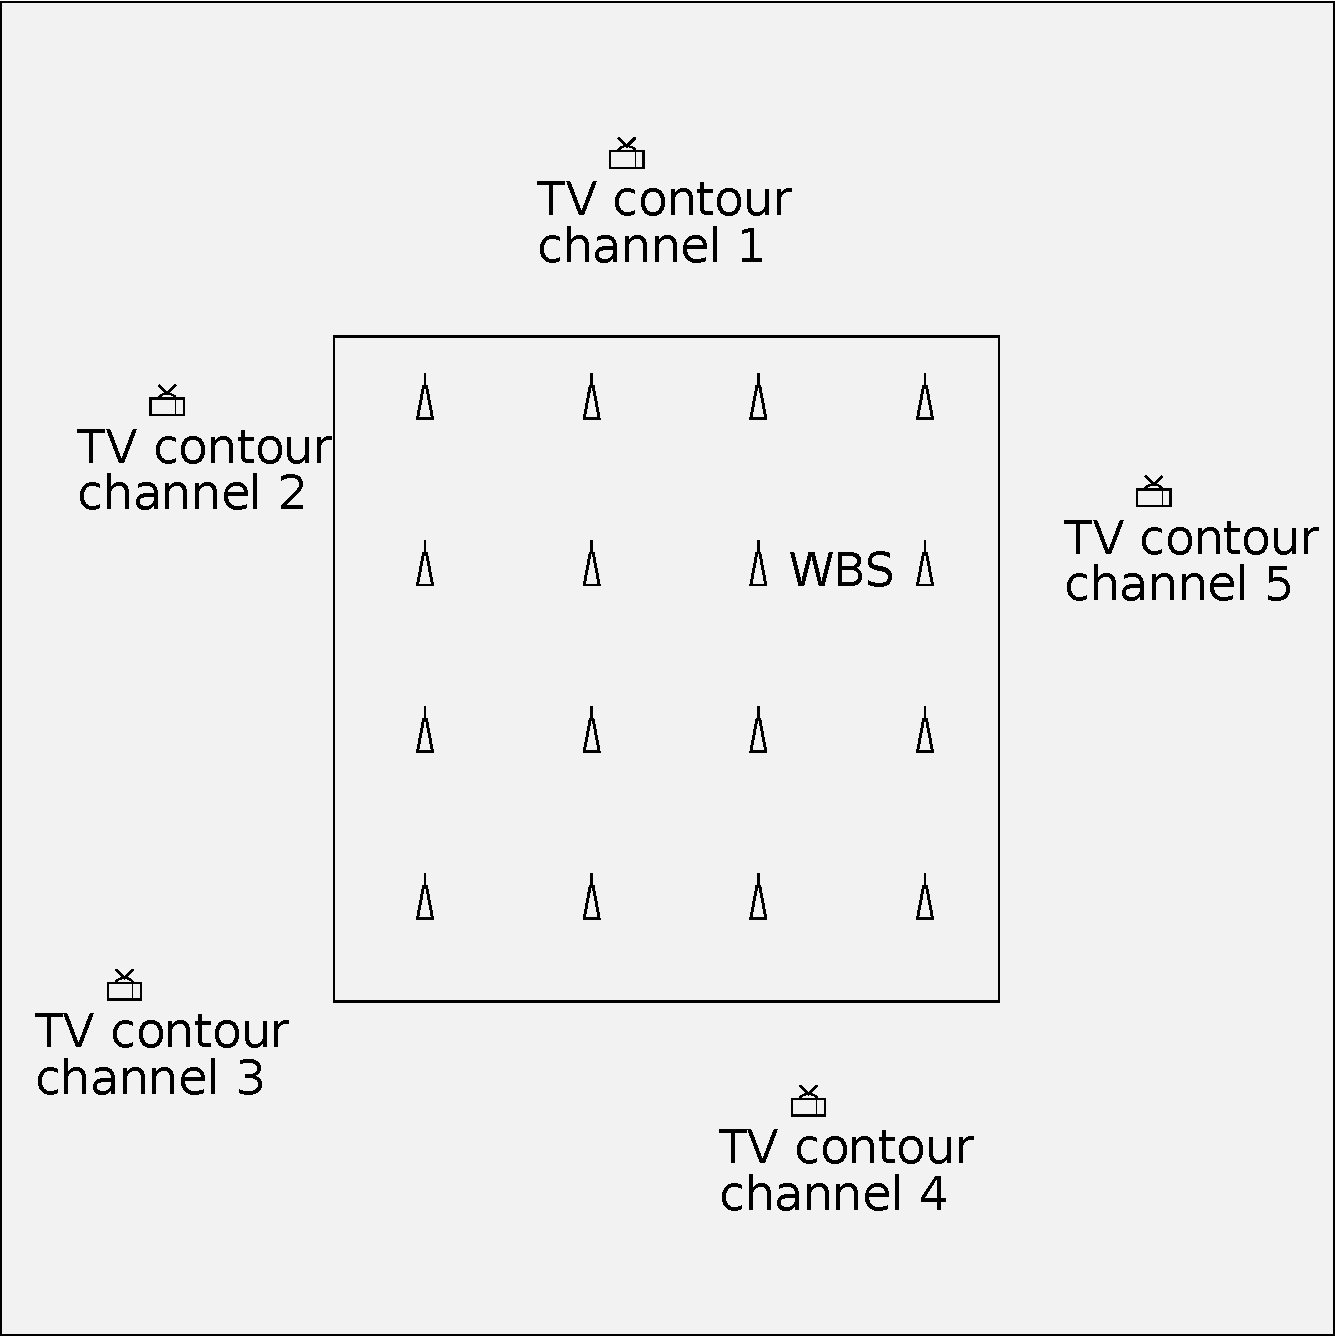
\includegraphics[width=0.5\linewidth]{layout.pdf}
  \caption{Layout of WBSs and TV contours}
  \label{sim:layout}
\end{figure}

Some parameters are listed in Table~\ref{6}.

\begin{table}[!h]
\centering
\begin{tabular}{|l|r|}
  \hline
  Number of channels 						& 5 \\
  Number of WBSs							& 16\\
  Noise 									& $10^{-12}$W \\ % -90dbm
  Length of side the square to locate WBSs		& 60km\\
  Distance between quasai terminal and WBS 	& 7km \\
  Interference threshold on TV contour 		& $10^{-7}$W \\ % -67dbm
  Path loss factor 							& 2 \\
  Standard deviation in flat shadowing		& 8\\
  Number of end terminals in network 		& 800 \\
  Min. WBS Tx power~\footnotemark{} complying with ECC 			& 1W \\
  Max. WBS Tx power complying with ECC			& 20W \\
  $P_{\mathtt{op}}$, Tx power complying with FCC   & 4W\\

  \hline
\end{tabular}
\caption{Simulation parameters}
\label{simulationparameter}
\end{table}
\footnotetext{minimal and maximal power here denote the power level restricted by the specification of hardware.}

\subsection{Schemes Complying with ECC Regulations}
\label{MaxPower_whitecat}

%In this section, we will firstly evaluate the convex optimization and linear optimization proposed in Section~\ref{powermap} to see which is the better choice to decide the maximum permitted transmission power, the adopted metrics are average power consumption, and SINR on end users where channel allocation is executed.
We compare \textit{whiteCat} with centralized scheme and three other distributed schemes: the random allocation scheme, \textit{whiteCase} and No-regret learning.

\begin{itemize}
\item \textit{Optimization}: centralized quadratic optimization introduced in Section~\ref{03_centralized_ca}.

\item \textit{WhiteCase}:  \underline{White}space \underline{c}hannel \underline{a}llocation \underline{se}lfish, where WBSs minimize only the first item of Formula~\ref{utility}

\item \textit{Potential Game}: A potential game based distributed scheme which is introduced in~\cite{pimrc_2012}.

\item \textit{No-Regret Learning}: A distributed scheme introduced in \cite{hart00correlatedeq}.

\item \textit{Random Scheme}: WBS choose channel randomly.


\end{itemize}


\subsubsection{The Choice of Radius of Auxiliary Circles, quasiSINR of WBS, and SINR on End Users}
The usage of quasiSINR exempts WBSs from taking care the SINR on the end terminals.
A WBS's quasiSINR is related with WBS's location and the radius of auxiliary circle.
Figure~\ref{radius} illustrates the effect of using different radii of the auxiliary circle on the data rate can be achieved by end terminals.

\begin{figure}[h]
\centering
\subfigure[quasiSINR of WBSs]{
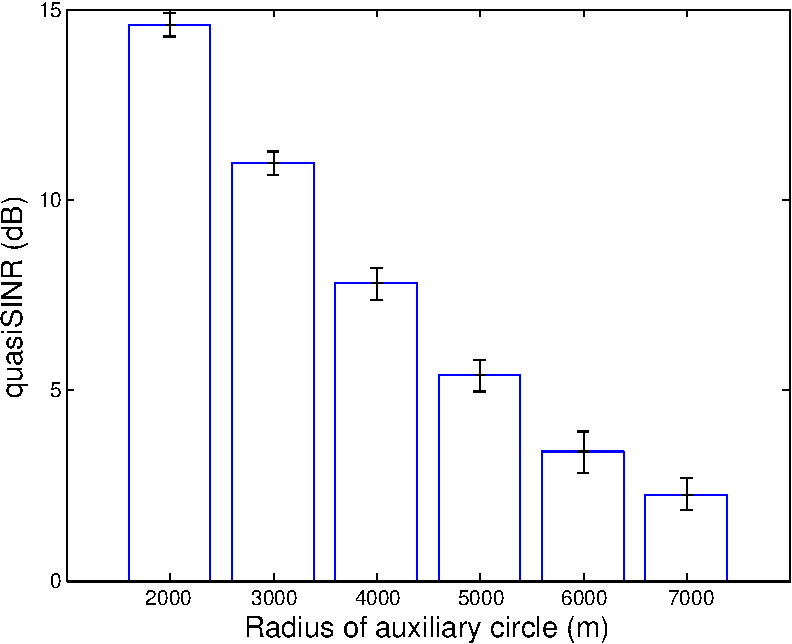
\includegraphics[width=0.435\linewidth]{qusaiSINR_with_radius.pdf}
\label{qusaiSINR_with_radius}
}
\subfigure[Data rate of end terminals when applying whiteCat]{
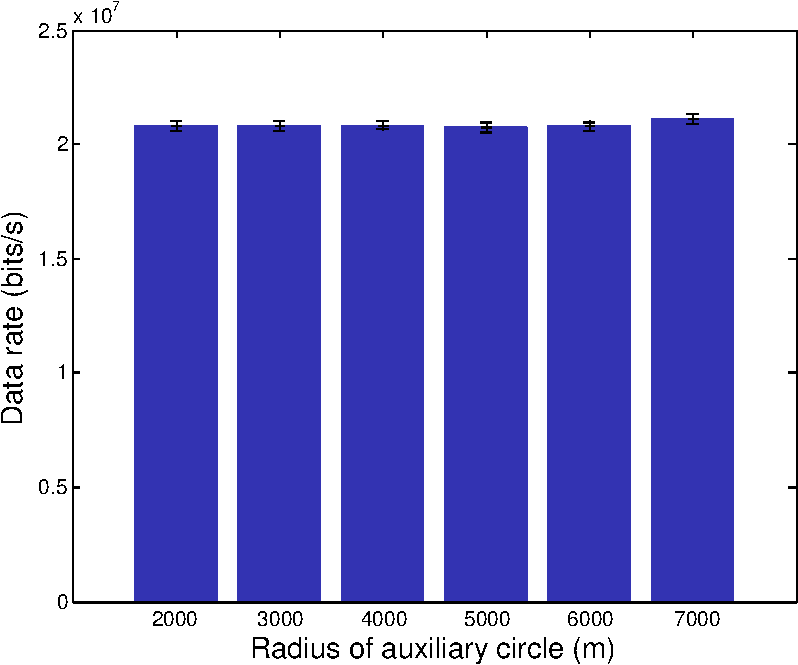
\includegraphics[width=0.435\linewidth]{sinr_on_endusers_with_radius.pdf}
\label{sinr_on_endusers_with_radius}
}
\caption[]{The effects of different radii of auxiliary circle on end terminals' data rate. Maximum permitted power is obtained by solving convex optimization. WhiteCat is used to assign the channels.}
\label{radius}
\end{figure}

Subfigure~\ref{qusaiSINR_with_radius} shows WBSs' quasiSINR decreases when the radii of auxiliary circles increase.
Subfigure~\ref{sinr_on_endusers_with_radius} illustrates the choice on radius of auxiliary circle don't influence the performance of whiteCat.
In the following simulation, we fixed the radius at 6000 m.

\subsubsection{Comparison of Schemes Complying with ECC Regulations}
 
Figure~\ref{transPower} depicts the transmission power consumption of the schemes.
whiteCat and the optimization method consume the less energy than the potential game scheme and random scheme.
whiteCat and the optimization method consume more energy than No-Regret learning scheme and WhiteCase, but meanwhile the former two schemes output the latter two in terms of SINR which will be shown in Figure~\ref{6000_sinr}.

 \begin{figure}[h!]
    \centering
      \includegraphics[width=0.9\linewidth]{ECC_aveageTxPOverChannels.pdf}
    \caption{Average Transmission power of WBSs when different number of channels are available}
\label{transPower}    
  \end{figure}
  
 %Figure~\ref{qusaiSINR} shows the quasiSINR of WBSs.
%The centralized optimization scheme achieves the highest quasiSINR, because the optimization formulation~\ref{QLP} obtains the global optima.

%   \begin{figure}[h!]
%       \centering
%       \includegraphics[width=0.9\linewidth]{ECC_16_4_5e1-8_5000_1_20_10_qusaiSINR.pdf}
%       \caption{QuasiSINR of WBSs achieved by different distributed spectrum allocation schemes under different ways deciding the maximal transmission power map}
%	\label{qusaiSINR}
%     \end{figure}
     
The average SINR on the end terminals is depicted in Figure~\ref{6000_sinr}.
whiteCat and the centralized optimization achieve similar and the best performance among the schemes.
The potential game based scheme and random scheme achieve good SINR with the cost of hight transmission power.
WhiteCase and No-Regret learning are at the bottom.
     \begin{figure}[h!]
       \centering
       \includegraphics[width=0.9\linewidth]{ECC_SINR_overChannels.pdf}
       \caption{SINR on end terminals}
	\label{6000_sinr}
     \end{figure}

%  \begin{figure}[h!]
%     \centering
%     \includegraphics[width=0.8\linewidth]{ECC_SINRCdf.pdf}
%     \caption{CDF of SINR on end users}
%     \label{6000_sinr_cdf}
%  \end{figure}
%The empirical cumulative distribution function curve of SINR on end terminals is drawn in Figure \ref{6000_sinr_cdf}.
%The SINR achieved by WhiteCat and the centralized optimization is stably higher than that obtained from other schemes.
%For example, the 20\% and 80\% percentile of the SINR achieved by WhiteCat and the centralized optimization are 0.5 to 1 dB higher than the other channel allocation schemes.






\subsubsection{Convergence Speed}

%Complexity: 
%For each player, there are at most $(n-1)*|\mathbb{C}|$ resources available for usage, while, because the produced congestion on each resource is independent on channel, in other words, the congestions involving the same pair of players are quantitatively identical, there are only $(n-1)$ quantitatively different congestions on one player's resources. So, the number of combinations with quantitatively non-identical congestions involved with that player is $2^{(n-1)}$, accordingly there are totally $n*2^{(n-1)}$ quantitatively different congestions for the whole the problem. We adopt the method of \cite{LectureA}, which resorts the congestions in a increasing sequence, and replaces the original congestions with integer values starting form 1. We call the integers as \textit{new} congestions. In this way the preferences of the players are preserved and we can find easily the biggest possible congestion is $n*2^{(n-1)}$, which is the upper bound for the number of steps towards convergence.
In the congestion game where scheme whiteCat is derived, each player (WBS) has at most $(n-1)*|\mathbb{C}|$ resources available for usage, thus there is no polynomial steps converging to NE, while, simulation shows the algorithm can quickly converge to NE when the number of WBS is up to 100. 
%Figure \ref{100converge} shows that for 100 WBSs, whitecat executes at most 5 iterations (in one iteration all WBSs update their choices). 
%Figure \ref{convergeComp} depicts one instance of simulation, where whiteCat converges quickly, No-regret produces oscillation but converges finally, while WhiteCase can not converge thus has to be enforced stop after 16000 updates. %\todo{replot}%, whereas 
%
Table~\ref{convergencespeed} shows the average number of steps needed before convergence in 100 runs of simulations.
As to whiteCat, we account each WBS accessing the base station (refer to \ref{whitecat}) as \textit{one step}.
We compare the convergence speed of WhteCat with no-regret learning, the scheme derived from potential game~\cite{pimrc_2012} and whiteCase.
Note that the potential game scheme is to solve joint power and channel allocation problem, as it is developed with game theory, it is reasonable to see its convergence speed.
As there is no guarantee for WhiteCase to converge, we stop the channel allocation process after 16000 steps (1000 rounds).

Table~\ref{convergencespeed} tells that whiteCat is two times faster than the scheme derived from potential game, and 20 times faster than no-regret learning scheme.
The relatively smaller confidence interval shows that whiteCat's convergence is not affected by different network configurations.
Fast converge is attributed to the working style of WBSs whcih access the database to get the information of other WBSs, thus the distributable decision involves a part of the global information of the network.
Thus, we can see that the speed up of convergence is due to the overhead caused by accessing the database.


Figure \ref{convergeComp} depicts one instance of the convergence processes of three schemes.
The Y axis is the summed utility of all WBSs.
We can see whiteCat decreases the summed utility constantly, and the channel allocation process ceases after 38 times of updates.
Whereas, noregret learning scheme takes 120 steps before convergence, and whiteCase fails to converge.
%XXXXXX ***************
%Notice that there is a slight rise when the value on the X-axis is 35, which comes from the difference between \ref{compare} and \ref{allPotential}.
%XXXXXX ***************
\begin{table}[!h]
\centering
\begin{tabular}{|l|c|c|c|}
  \hline
  Scheme			 						& Average  	 		& 95\% CI			&Average \\
  												& steps					&							&time (s) \\
    \hhline{|=|=|=|=|}
  WhiteCat									& 58						& 5.6						&2\\\hline
  No-Regret Learning									& 1916						& 1541						&144\\\hline
  Potential Game~\cite{pimrc_2012}			& 120						& 10						&4\\\hline
  Optimization						& -                         & -                         &40\\\hline
  WhiteCase 								& 4587 						& 2742						&50\\  
  \hline
\end{tabular}
\caption{Convergence speed of the distributed channel allocation schemes. As to the distributed scheme, the time involved to communicate with database is note considered and included.}
\label{convergencespeed}
\end{table}

%\begin{figure}[h!]
%\label{100converge}
%  \centering
%  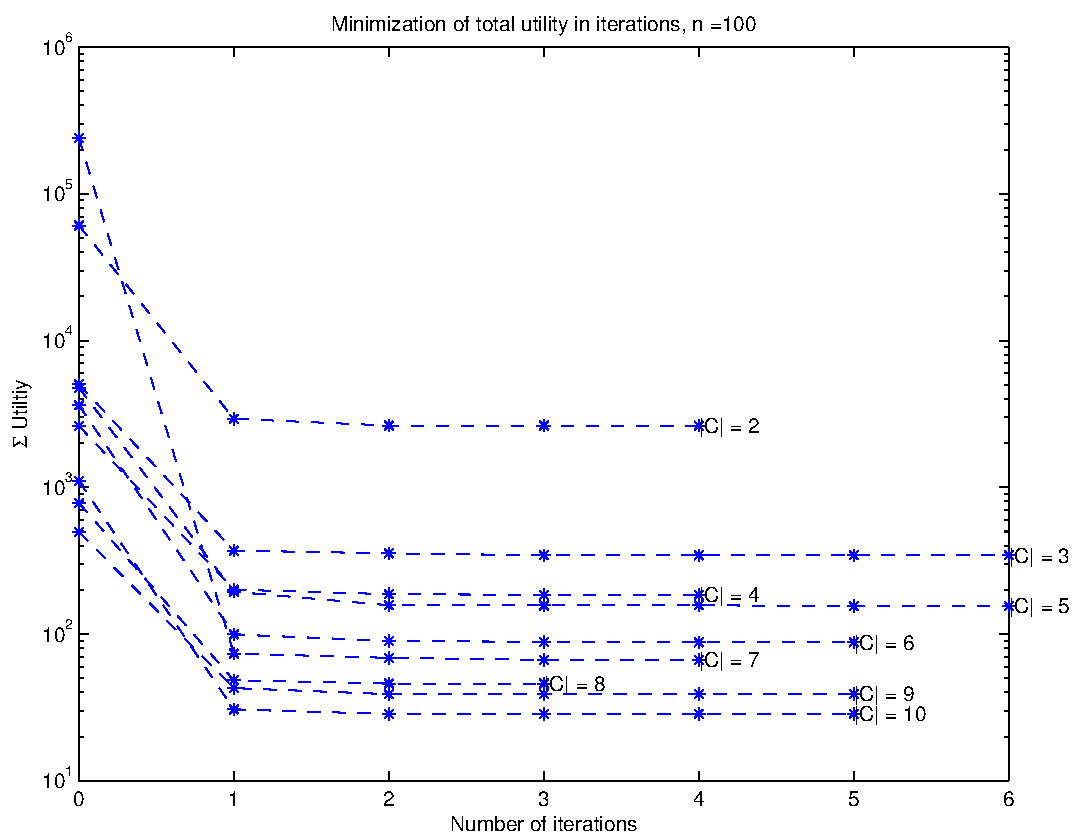
\includegraphics[width=0.65\linewidth]{CAConverenge100.pdf}
%  \caption{100 WBSs, 2-10 channels}
%\end{figure}

\begin{figure}[h!]
  \centering
  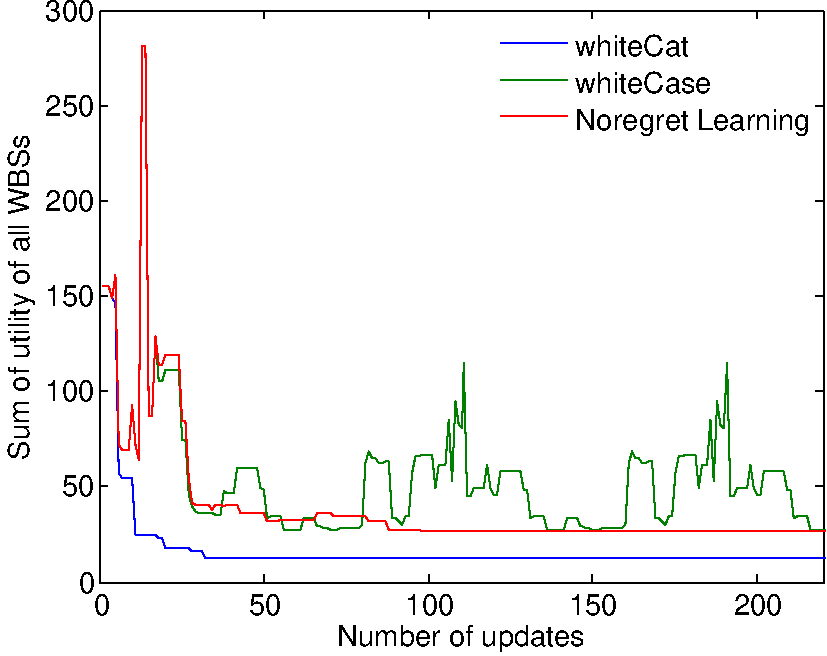
\includegraphics[width=0.8\linewidth]{convergence.pdf}
  \caption{Convergence process of three different schemes in one simulation.}
\label{convergeComp}
\end{figure}




%\subsubsection{Stability of SINR in Convergence Process}
%WBS provides service to end users in the process of channel allocation. 
%A certain SINR corresponds to certain transmission configurations like modulation type and data rate. 
%The oscillation of SINR resulted from WBS changing the working channel during the convergence process may cause reconfiguration, reduced throughput or delay variance, which is not preferred.
%We propose a metric \textit{Cost of Oscillation} (COS) to represent the stability of SINR in the converging process.
%Assuming each update of channel takes 1 time unit, the variance of SINR of end user $i$ at time $t+1$ is \[\varDelta  \gamma_i(t+1)=\mid\frac{\gamma_i(t+1)-\gamma_i(t)}{\gamma_i(t)} \mid\]. 
%
%The COS value for one network applied with a certain channel allocation scheme is,
%\begin{equation}
%\label{cos}
%			COS = \sum\limits_{t=1}^T   \sum\limits_{i\in \mathcal{N}} \varDelta  \gamma_i(t)
%			\end{equation}
%$\gamma_i(0)$ is the SINR for $i$ before starting channel allocation.
%The variance of SINR in channel allocation process is shown in table \ref{costable} from which we can see WhiteCat achieves only 6\% of oscillation on SINR compared with No-regret approach.
%\begin{table}[!h]
%\centering
%\begin{tabular}{|l|c|c|}
%  \hline
%  Scheme			 						& COS 					& 95\% confidence interval\\
%    \hhline{|=|=|=|}
%  WhiteCat									& 8850					& 2984\\\hline
%  No-Regret Learning									& 145460				& 1541\\\hline
%  WhiteCase 								& 246790 				& 168050\\ 
%  \hline
%\end{tabular}
%\caption{Variance of SINR during the convergence process}
%\label{costable}
%\end{table}



\subsection{Schemes for FCC Regulations}
\label{performance_FCC}

Figure~\ref{sumOfUtility} shows the utilities obtained by optimization is larger than the distributed scheme.
The major reason is for the distributed scheme, some WBSs are allowed to be idle, in comparison, every WBS in optimization must operate with either $P_\mu$ or  $P_{\mathtt{op}}$ and the utility becomes large when the transmission power is $P_\mu$.
\begin{figure}[h!]
  \centering
      \includegraphics[width=0.8\linewidth]{FCC_sumUtility.pdf}
  		\caption{Sum of Utility}
     \label{sumOfUtility}
\end{figure}

Figure~\ref{FCCSINREndUsers} illustrates the average SINR on end users, where the distributed scheme outperforms the centralized scheme.
Figure~\ref{FCCSINRCdf} provides another perspective for the SINR on the end users.
From the figure we can see, 95\% percent of end terminals have SINR between 1 to 80 dB, and more than 90\% have SINR which is higher than 4 dB.
In particular, with the centralized scheme 97\% of end terminals have SINR which is lower than 20 dB, in comparison, with the distributed scheme, this percentage is 87\% and the rest of end terminals have SINR which is higher than 20 dB.
%\begin{figure}[h!]
%  \centering
%  \includegraphics[width=0.8\linewidth]{FCC_qusaiSINR.pdf}
%  \caption{QuasiSINR}
%\label{FCCQuasiSINR}
%\end{figure}

\begin{figure}[h!]
  \centering
      \includegraphics[width=0.8\linewidth]{FCC_SINR_endUsers.pdf}
  		\caption{Average SINR on end users}
     \label{FCCSINREndUsers}
\end{figure}


\begin{figure}[h!]
  \centering
      \includegraphics[width=0.8\linewidth]{FCC_SINRCdf.pdf}
  		\caption{Cumulative distribution of SINR on end users after channel and power allocation}
     \label{FCCSINRCdf}
\end{figure}

In terms of power consumption as shown in Figure~\ref{FCCTxpower}, the distributed scheme consumes only 76\% of the centralized optimization.
The reason is explained in Figure~\ref{FCC_N_operatingWBSs} \ie by executing the former scheme, more WBSs are allowed to be idle than the latter.

\begin{figure}[h!]
  \centering
  \includegraphics[width=0.8\linewidth]{FCC_aveageTxP.pdf}
  \caption{Average transmission power of one WBS}
\label{FCCTxpower}
\end{figure}

\begin{figure}[h!]
  \centering
  \includegraphics[width=0.8\linewidth]{FCC_N_operatingWBSs.pdf}
  \caption{Number of WBSs operating with $P_{\mathtt{op}}$}
\label{FCC_N_operatingWBSs}
\end{figure}





\section{Conclusions}
In this paper, we look into the channel allocation problem in TV white space with respect to ECC and FCC regulations respectively.
Both centralized and distributed solutions are proposed. 
In particular, we improve the SINR on the end terminals in the cells.
Under the ECC rules, the proposed centralized scheme obtains the global optimal.
In comparison, the congestion game based distributed scheme achieves comparable performance in terms of end user SINR and power consumption, but it outperforms other distributed schemes in terms of end user SINR and algorithm execution speed.
With respect to the TV spectrum usage under FCC rules, we for the first time investigate the problem of channel allocation in order to improve the SINR on end users, where the TV systems could be interfered by the aggregated interference.
Proposed centralized scheme achieves the global optimal after linear relaxizaiton, and the proposed distributed scheme is proved to converge by congestion game theory, and the simulation shows the distributed scheme outperforms the centralized scheme in terms of power consumption and SINR on end users.




\bibliography{../backmatter/myrefs}
\bibliographystyle{IEEEtran}
\end{document}